\documentclass[11pt,a4paper]{article}
% --------------------------------------------------
% Encodage et langue
% --------------------------------------------------
\usepackage[utf8]{inputenc}
\usepackage[T1]{fontenc}
\usepackage[french]{babel}
\usepackage{lmodern}
\usepackage{microtype}

% --------------------------------------------------
% Mise en page
% --------------------------------------------------
\usepackage[a4paper, margin=2.5cm]{geometry}
\usepackage{setspace}
\onehalfspacing

% --------------------------------------------------
% Mathématiques
% --------------------------------------------------
\usepackage{amsmath}
\usepackage{amssymb}
\usepackage{amsfonts}
\usepackage{mathtools}

% --------------------------------------------------
% Figures, tableaux et couleurs
% --------------------------------------------------
\usepackage{graphicx}
\usepackage{float}
\usepackage{booktabs}
\usepackage{tabularx}
\usepackage{longtable}
\usepackage{multirow}
\usepackage{array}
\usepackage[table]{xcolor}
\usepackage{caption}
\usepackage{subcaption}

% --------------------------------------------------
% Liens
% --------------------------------------------------
\usepackage[hidelinks]{hyperref}
\usepackage[nameinlink,noabbrev]{cleveref}

% --------------------------------------------------
% Code source
% --------------------------------------------------
\usepackage{listings}

\definecolor{codebackground}{RGB}{248,248,248}
\definecolor{codekeyword}{RGB}{0,70,140}
\definecolor{codecomment}{RGB}{0,120,70}
\definecolor{codestring}{RGB}{170,50,0}
\definecolor{codegray}{RGB}{100,100,100}

\lstdefinestyle{pythonstyle}{
    language=Python,
    backgroundcolor=\color{codebackground},
    basicstyle=\ttfamily\small,
    keywordstyle=\color{codekeyword}\bfseries,
    commentstyle=\color{codecomment},
    stringstyle=\color{codestring},
    numberstyle=\tiny\color{codegray},
    numbers=left,
    numbersep=8pt,
    frame=single,
    framerule=0.3pt,
    breaklines=true,
    breakatwhitespace=false,
    showstringspaces=false,
    tabsize=4,
    columns=fullflexible,
    captionpos=b
}

\lstset{style=pythonstyle}

% --------------------------------------------------
% TikZ : diagrammes d'architecture
% --------------------------------------------------
\usepackage{tikz}
\usetikzlibrary{
    arrows.meta,
    positioning,
    shapes.geometric,
    fit,
    backgrounds,
    calc
}

\tikzset{
    module/.style={
        rectangle,
        rounded corners,
        draw=blue!60!black,
        fill=blue!8,
        minimum width=3.2cm,
        minimum height=1cm,
        align=center,
        font=\small
    },
    component/.style={
        rectangle,
        rounded corners,
        draw=green!50!black,
        fill=green!8,
        minimum width=2.6cm,
        minimum height=0.8cm,
        align=center,
        font=\small
    },
    arrow/.style={
        -{Latex[length=3mm]},
        thick
    }
}

% --------------------------------------------------
% Commandes utiles
% --------------------------------------------------
\newcommand{\AUSSI}{\textsc{AUSSI V2}}
\newcommand{\BFS}{\textsc{BFS}}
\newcommand{\UCS}{\textsc{UCS}}
\newcommand{\Greedy}{\textsc{Greedy}}
\newcommand{\AStar}{\textsc{A*}}
\newcommand{\TreeSearch}{\textsc{Tree-Search}}
\newcommand{\GraphSearch}{\textsc{Graph-Search}}

\newcommand{\code}[1]{\texttt{#1}}

% --------------------------------------------------
% Style des sections
% --------------------------------------------------
\usepackage{titlesec}

\titleformat{\section}
    {\Large\bfseries}
    {\thesection}
    {0.8em}
    {}

\titleformat{\subsection}
    {\large\bfseries}
    {\thesubsection}
    {0.7em}
    {}

% --------------------------------------------------
% Colonnes de tableau
% --------------------------------------------------
\newcolumntype{Y}{>{\raggedright\arraybackslash}X}
\newcolumntype{C}{>{\centering\arraybackslash}X}

\begin{document}
\shorthandoff{:}
\pagenumbering{roman}

\begin{titlepage}
    \centering
    \vspace*{1.2cm}
    {\scshape\Large Université du Québec à Chicoutimi\par}
    \vspace{0.4cm}
    {\scshape\large 8INF878 -- Intelligence artificielle agentique\par}
    \vspace{2cm}
    {\Huge\bfseries AUSSI V2\par}
    \vspace{0.3cm}
    {\LARGE\bfseries Résolution de problèmes et généralisation\par}
    \vspace{1.5cm}
    {\Large Travail pratique no 1\par}
    \vfill
    \begin{tabular}{rl}
        \textbf{Équipe :} & SIDIBÉ Doriane \\
                          & Kanyinda Kalonji Germain \\
                          & Astride Melvin Fokam Ninyim \\
                          & Lionnel Cedric Nana Leunkeu \\
        \\
        \textbf{Cours :} & 8INF878 -- Intelligence artificielle agentique \\
        \textbf{Professeur :} & Kevine Bouchard \\
        \textbf{Date de remise :} & 9 octobre 2026 \\
    \end{tabular}
    \vfill
    {\large Saguenay, Québec, Canada\par}
    {\large Automne 2026\par}
\end{titlepage}

\begin{abstract}
Ce rapport présente \AUSSI{}, un moteur générique de résolution de problèmes
fondé sur la recherche dans un espace d'états. Le système utilise un moteur
commun pour les labyrinthes, la navigation, le N-Puzzle et le jeu arithmétique,
avec les stratégies \BFS{}, \UCS{}, \Greedy{} et \AStar{} et les modes
\TreeSearch{} et \GraphSearch{}. Une évaluation ciblée de 44 exécutions compare
les coûts de solution, les noeuds générés et expansés, la taille de la
frontière et les temps mesurés. Les résultats illustrent notamment l'influence
de la stratégie, de la mémorisation des états et du choix d'heuristique.
\end{abstract}

\noindent\textbf{Mots-clés :}
recherche informée, \AStar{}, \BFS{}, \UCS{}, \Greedy{},
heuristique, \TreeSearch{}, \GraphSearch{}, espace d'états.

\tableofcontents
\clearpage
\pagenumbering{arabic}

\section{Introduction}

Les agents intelligents doivent souvent résoudre des problèmes dont la structure
varie fortement : trouver un chemin dans une grille, planifier un itinéraire
routier, réorganiser un puzzle ou construire une expression arithmétique.
Malgré cette diversité, ces tâches peuvent être formulées comme des problèmes
de recherche dans un espace d'états.

L'objectif de ce travail est de concevoir \AUSSI{}, un moteur générique de
résolution de problèmes. Le système doit permettre de résoudre plusieurs types
de problèmes sans modifier les algorithmes d'exploration. Seules la formulation
du problème et, lorsque nécessaire, l'heuristique doivent varier.

Le moteur implémente les stratégies \BFS{}, \UCS{}, \Greedy{} et \AStar{}.
Il permet aussi de choisir entre les modes \TreeSearch{} et \GraphSearch{}.
Les problèmes pris en charge sont les labyrinthes, la navigation dans un graphe
pondéré, le N-Puzzle et le jeu arithmétique.

Les contributions principales du projet sont les suivantes :

\begin{itemize}
    \item Une interface générique \code{Problem} indépendante des domaines.
    \item Un moteur unique \code{SEARCH(problem, strategy, mode)}.
    \item Des stratégies de recherche interchangeables.
    \item Une gestion configurable des états répétés.
    \item Une interface utilisateur permettant de sélectionner un problème,
    une stratégie et un mode de recherche.
    \item Une collecte systématique des métriques d'exécution.
    \item Une étude comparative des algorithmes sur plusieurs instances.
\end{itemize}

Le reste du rapport présente les exigences du projet, l'architecture proposée,
la modélisation des problèmes, les algorithmes implantés, l'interface, les
expériences réalisées et une discussion des résultats.
\section{Analyse des exigences}

Le mandat demande la construction d'un agent généraliste de résolution de
problèmes. L'objectif n'est donc pas de programmer quatre solveurs indépendants,
mais de construire un moteur de recherche réutilisable pour plusieurs espaces
d'états.

Le \cref{tab:exigences} relie chaque exigence fonctionnelle à la décision de
conception adoptée dans \AUSSI{}.

\begin{table}[H]
\centering
\caption{Correspondance entre les exigences et la conception proposée.}
\label{tab:exigences}
\begin{tabularx}{\textwidth}{p{4cm}Y}
\toprule
\textbf{Exigence} & \textbf{Réponse de conception} \\
\midrule
BFS, UCS, Greedy et A* &
Les stratégies sont définies par une politique de priorité interchangeable. \\
\addlinespace

Tree-Search et Graph-Search &
Le moteur accepte un mode de recherche qui contrôle la gestion des états
visités et des chemins répétés. \\
\addlinespace

Moteur générique &
La fonction \code{SEARCH(problem, strategy, mode)} dépend seulement de
l'interface abstraite \code{Problem}. \\
\addlinespace

Quatre catégories de problèmes &
Chaque domaine implémente les opérations génériques : état initial, actions,
transition, test de but, coût et heuristique. \\
\addlinespace

Interface utilisateur &
Une interface en ligne de commande permet de choisir le problème, l'instance,
la stratégie, le mode et certaines limites de ressources. \\
\addlinespace

Statistiques &
Chaque exécution retourne un objet \code{SearchResult} contenant le statut,
la solution, le coût, la profondeur et les métriques d'exécution. \\
\addlinespace

Expérience comparative &
Un protocole de benchmark exécute plusieurs instances et exporte les résultats
dans un format tabulaire reproductible. \\
\bottomrule
\end{tabularx}
\end{table}

\subsection{Objectif de généralisation}

Le principe central de \AUSSI{} est de séparer les éléments invariants des
éléments spécifiques à un problème. Les éléments invariants sont le moteur de
recherche, la gestion de la frontière \code{OPEN}, la construction des noeuds,
la collecte des métriques et la reconstruction de solution.

Les éléments variables sont la représentation d'état, les actions disponibles,
la fonction de transition, le test de but, les coûts et l'heuristique. Cette
séparation permet d'ajouter un nouveau problème sans réécrire les algorithmes
de recherche.
\section{Architecture du système}

\subsection{Vue d'ensemble}

L'architecture de \AUSSI{} repose sur la séparation entre le moteur de
recherche générique et les problèmes particuliers. Le moteur reçoit un objet
respectant l'interface \code{Problem}, une stratégie de recherche et un mode
de gestion des états.

La fonction centrale du système est définie comme suit :

\begin{center}
\code{SEARCH(problem, strategy, mode)}
\end{center}

\begin{figure}[H]
\centering
\begin{tikzpicture}[node distance=1.1cm and 1.3cm]

\node[module] (ui) {Interface utilisateur\\CLI};
\node[module, right=of ui] (search) {Moteur générique\\\code{SEARCH()}};
\node[module, right=of search] (metrics) {Résultats et\\métriques};

\node[component, below=of search] (strategy) {Stratégie\\BFS / UCS / Greedy / A*};
\node[component, below=of ui] (mode) {Mode\\Tree / Graph};
\node[component, below=of metrics] (problem) {Problèmes\\Labyrinthe, navigation,\\N-Puzzle, arithmétique};

\draw[arrow] (ui) -- (search);
\draw[arrow] (search) -- (metrics);
\draw[arrow] (strategy) -- (search);
\draw[arrow] (mode) -- (search);
\draw[arrow] (problem) -- (search);

\end{tikzpicture}
\caption{Architecture générale de \AUSSI{}.}
\label{fig:architecture}
\end{figure}

\subsection{Interface \code{Problem}}

Tous les domaines respectent une même interface. Cette interface encapsule les
parties spécifiques à un problème de recherche.

\begin{lstlisting}[caption={Interface conceptuelle d'un problème.}, label={lst:problem-interface}]
class Problem:
    def initial_state(self):
        pass

    def is_goal(self, state) -> bool:
        pass

    def actions(self, state):
        pass

    def result(self, state, action):
        pass

    def step_cost(self, state, action, next_state) -> float:
        pass

    def heuristic(self, state) -> float:
        return 0.0

    def state_key(self, state):
        return state
\end{lstlisting}

La méthode \code{state\_key} fournit une représentation immuable et comparable
d'un état. Elle est utilisée par le mode \GraphSearch{} pour détecter les
états déjà rencontrés et conserver le meilleur coût connu.

\subsection{Noeud de recherche}

Un noeud de recherche contient au minimum l'état courant, un pointeur vers son
parent, l'action ayant produit l'état, le coût cumulé $g(n)$ et la profondeur.
Cette structure permet de reconstruire la solution après l'atteinte d'un état
but.

\begin{lstlisting}[caption={Structure conceptuelle d'un noeud de recherche.}]
@dataclass
class Node:
    state: Any
    parent: Node | None
    action: Any | None
    path_cost: float
    depth: int

    def solution(self):
        actions = []
        node = self
        while node.parent is not None:
            actions.append(node.action)
            node = node.parent
        return list(reversed(actions))
\end{lstlisting}

\subsection{Résultat standardisé}

Le moteur retourne un objet de résultat commun à tous les problèmes. Celui-ci
contient notamment le statut de résolution, le chemin, le coût, la profondeur,
le nombre de noeuds générés, le nombre de noeuds expansés, la taille maximale
de la frontière et le temps d'exécution.
\section{Modélisation des problèmes}

Chaque problème est décrit à partir des mêmes composantes : état, actions,
fonction de transition, test de but, coût et heuristique.

\begin{table}[H]
\centering
\caption{Résumé de la modélisation des quatre problèmes.}
\label{tab:modelisation}
\begin{tabularx}{\textwidth}{p{2.4cm}Y Y Y}
\toprule
\textbf{Problème} & \textbf{État} & \textbf{Actions} & \textbf{Heuristique} \\
\midrule
Labyrinthe &
Position courante $(r,c)$ &
Déplacements valides vers les cellules voisines &
Distance de Manhattan jusqu'à l'objectif \\
\addlinespace

Navigation &
Ville courante &
Emprunter une route adjacente &
Distance euclidienne à vol d'oiseau \\
\addlinespace

N-Puzzle &
Configuration des tuiles &
Déplacement de la case vide &
Somme des distances de Manhattan des tuiles \\
\addlinespace

Jeu arithmétique &
Valeurs restantes et expressions associées &
Choisir deux termes et appliquer une opération &
Heuristique spécifique ou nulle selon l'instance \\
\bottomrule
\end{tabularx}
\end{table}

\subsection{Labyrinthe}

Dans le problème du labyrinthe, un état est une position $(r,c)$ dans une
grille. Les actions correspondent aux déplacements vers le haut, le bas, la
gauche et la droite, sous réserve que la cellule cible soit accessible.

Lorsque les déplacements sont orthogonaux, l'heuristique de Manhattan est
définie par :

\[
h(n) = |r_n - r_G| + |c_n - c_G|
\]

Dans le cas d'un labyrinthe pondéré, une version admissible peut être obtenue
en multipliant cette distance par le plus faible coût de déplacement possible.

\subsection{Navigation}

Le problème de navigation est représenté par un graphe pondéré. Chaque ville
possède des coordonnées simplifiées $(x,y)$ et les arêtes représentent les
routes disponibles. Le coût d'une action correspond au poids de la route
empruntée.

L'heuristique utilisée est la distance euclidienne à vol d'oiseau :

\[
h(n) =
\sqrt{(x_n-x_G)^2 + (y_n-y_G)^2}
\]

Pour préserver l'admissibilité, les coûts des routes doivent être cohérents
avec les distances géographiques ou être supérieurs à celles-ci.

\subsection{N-Puzzle}

Un état du N-Puzzle est représenté par un tuple immuable contenant la position
de chaque tuile. Les actions possibles déplacent la case vide vers une position
adjacente. Le coût de chaque déplacement est uniforme.

L'heuristique principale est la somme des distances de Manhattan des tuiles
vers leur position cible :

\[
h(s) = \sum_{t \neq 0}
\left(
|r_t-r_t^\star| + |c_t-c_t^\star|
\right)
\]

La case vide, notée $0$, est exclue de cette somme. Le système vérifie aussi
la solvabilité de l'instance avant de lancer une recherche potentiellement
coûteuse.

\subsection{Jeu arithmétique}

Dans le jeu arithmétique, un état contient les valeurs restantes ainsi que les
expressions permettant de les produire. Une action consiste à sélectionner deux
valeurs et à appliquer une opération parmi $+$, $-$, $\times$ et $\div$.

Les fractions exactes sont utilisées afin d'éviter les erreurs d'arrondi liées
aux nombres à virgule flottante. Les divisions par zéro sont interdites. Une
solution est atteinte lorsqu'une valeur restante est égale à la valeur cible.

\section{Algorithmes de recherche}

\subsection{Fonctions de priorité}

Les stratégies de recherche sont différenciées principalement par la fonction
utilisée pour ordonner la frontière \code{OPEN}. Le \cref{tab:priorites}
présente les fonctions de priorité implantées.

\begin{table}[H]
\centering
\caption{Fonctions de priorité des stratégies de recherche.}
\label{tab:priorites}
\begin{tabular}{lll}
\toprule
\textbf{Stratégie} & \textbf{Priorité} & \textbf{Interprétation} \\
\midrule
\BFS{} & $f(n)=\mathrm{depth}(n)$ & Explore par niveau de profondeur \\
\UCS{} & $f(n)=g(n)$ & Favorise le coût cumulé minimal \\
\Greedy{} & $f(n)=h(n)$ & Favorise l'état estimé le plus proche du but \\
\AStar{} & $f(n)=g(n)+h(n)$ & Combine coût passé et estimation restante \\
\bottomrule
\end{tabular}
\end{table}

\subsection{Breadth-First Search}

\BFS{} explore les noeuds dans l'ordre croissant de profondeur. Lorsque tous
les coûts d'action sont identiques, l'algorithme trouve une solution de
profondeur minimale. Cependant, il ne garantit pas une solution de coût minimal
dans un environnement pondéré.

\subsection{Uniform-Cost Search}

\UCS{} sélectionne le noeud avec le plus faible coût de chemin $g(n)$. Avec
des coûts d'action non négatifs, il retourne une solution de coût optimal.
Son principal inconvénient est que le nombre de noeuds explorés peut être élevé
lorsque l'espace d'états est important.

\subsection{Greedy Best-First Search}

La recherche gloutonne sélectionne le noeud ayant la plus faible valeur
heuristique $h(n)$. Elle peut trouver rapidement une solution si l'heuristique
est informative, mais elle ne garantit pas une solution optimale.

\subsection{A*}

\AStar{} utilise la fonction :

\[
f(n) = g(n) + h(n)
\]

Lorsque $h(n)$ est admissible, c'est-à-dire qu'elle ne surestime jamais le coût
réel restant, A* peut retourner une solution optimale. Une heuristique
consistante renforce ce comportement dans une recherche sur graphe.

\subsection{Tree-Search et Graph-Search}

En mode \TreeSearch{}, aucun mécanisme global n'empêche la génération répétée
d'un même état. Ce mode est simple, mais il peut être très coûteux en présence
de cycles ou de chemins convergents.

En mode \GraphSearch{}, le système conserve une structure \code{best\_g} qui
associe à chaque état le meilleur coût connu. Un noeud est ignoré si un chemin
strictement meilleur vers le même état a déjà été rencontré. Ce mécanisme réduit
les duplications et améliore généralement l'efficacité de la recherche.
\section{Interface utilisateur et présentation des résultats}

\subsection{Choix de configuration}

L'interface permet à l'utilisateur de choisir un problème, une instance, une
stratégie de recherche et un mode d'exploration. Des limites de temps ou de
nombre de noeuds peuvent aussi être configurées, notamment pour les instances
difficiles du N-Puzzle.

\begin{lstlisting}[caption={Exemple d'une session utilisateur.}]
=== AUSSI V2 ===

Probleme :
1. Labyrinthe
2. Navigation
3. N-Puzzle
4. Jeu arithmetique

> 1

Strategie :
1. BFS
2. UCS
3. Greedy Best-First
4. A*

> 4

Mode :
1. Tree-Search
2. Graph-Search

> 2
\end{lstlisting}

\subsection{Format de sortie}

Après une exécution, \AUSSI{} affiche les informations suivantes :

\begin{itemize}
    \item Le statut de l'exécution : solution trouvée, problème insoluble,
    limite de temps ou limite de noeuds atteinte.
    \item Le chemin ou la trace de raisonnement.
    \item Le coût total de la solution.
    \item La profondeur de la solution.
    \item Le nombre de noeuds générés.
    \item Le nombre de noeuds expansés.
    \item La taille maximale de la frontière \code{OPEN}.
    \item Le temps d'exécution.
\end{itemize}

\begin{lstlisting}[caption={Exemple de résultat affiché.}]
=== Resultat ===
Statut               : SOLVED
Strategie            : A*
Mode                 : Graph-Search
Cout total           : 18
Profondeur           : 14
Noeuds generes       : 86
Noeuds expanses      : 42
Taille maximale OPEN : 21
Temps                : 0.0038 s
Chemin               : R -> R -> D -> D -> ...
\end{lstlisting}

\subsection{Visualisation}

Pour les labyrinthes et les problèmes de navigation, la solution peut être
représentée visuellement. Dans le cas du N-Puzzle, les configurations
successives peuvent être affichées. Pour le jeu arithmétique, l'interface
présente l'expression finale et les opérations qui la composent.
\section{Expériences comparatives}
\label{sec:experiences}

\subsection{Protocole expérimental}

Un benchmark ciblé a été exécuté avec le moteur AUSSI V2 sur deux labyrinthes
(simple et pondéré), un trajet routier, un 8-Puzzle moyen et deux instances
arithmétiques (cible 24 et cible impossible 99). Les quatre stratégies
\BFS{}, \UCS{}, \Greedy{} et \AStar{} ont été évaluées. Les deux modes
\TreeSearch{} et \GraphSearch{} ont été comparés pour les labyrinthes; les
autres problèmes ont été exécutés en \GraphSearch{}. Une expérience
complémentaire compare, sur le même 8-Puzzle, trois heuristiques avec \AStar{} :
heuristique nulle, tuiles mal placées et distance de Manhattan.

Le jeu de données contient 44 exécutions. Pour chacune, le CSV conserve le
statut de résolution, le coût et la profondeur lorsqu'une solution est trouvée,
les noeuds générés et expansés, la taille maximale de \code{OPEN} et le temps
mesuré. \code{max\_open} est la taille maximale de la frontière; ce n'est pas
une mesure de la mémoire totale du processus. Chaque temps correspond à une
exécution unique et doit être interprété comme indicatif. Les nombres de noeuds
sont plus appropriés aux comparaisons reproductibles.

\subsection{Stratégies et gestion des états répétés}

La \cref{tab:maze-weighted} donne les résultats complets sur le labyrinthe
pondéré. Toutes les stratégies trouvent ici une solution de coût 9 et de
profondeur 6. Cette instance particulière ne départage donc pas les stratégies
sur le coût, mais met en évidence l'effet du mode de recherche sur l'effort.

\begin{table}[H]
\centering
\caption{Résultats sur le labyrinthe pondéré.}
\label{tab:maze-weighted}
\scriptsize
\begin{tabular}{llrrrrrr}
\toprule
\textbf{Stratégie} & \textbf{Mode} & \textbf{Gén.} & \textbf{Exp.} &
\textbf{OPEN max.} & \textbf{Coût / prof.} & \textbf{Résolue} &
\textbf{Temps (s)} \\
\midrule
BFS & Graphe & 32 & 13 & 3 & 9 / 6 & Oui & 0,000052 \\
BFS & Arbre & 203 & 85 & 118 & 9 / 6 & Oui & 0,000389 \\
UCS & Graphe & 37 & 15 & 3 & 9 / 6 & Oui & 0,000064 \\
UCS & Arbre & 1\,442 & 596 & 846 & 9 / 6 & Oui & 0,007855 \\
Greedy & Graphe & 23 & 9 & 4 & 9 / 6 & Oui & 0,000104 \\
Greedy & Arbre & 26 & 10 & 16 & 9 / 6 & Oui & 0,000162 \\
A* & Graphe & 30 & 12 & 5 & 9 / 6 & Oui & 0,000089 \\
A* & Arbre & 79 & 31 & 48 & 9 / 6 & Oui & 0,000189 \\
\bottomrule
\end{tabular}
\end{table}

\begin{figure}[H]
\centering
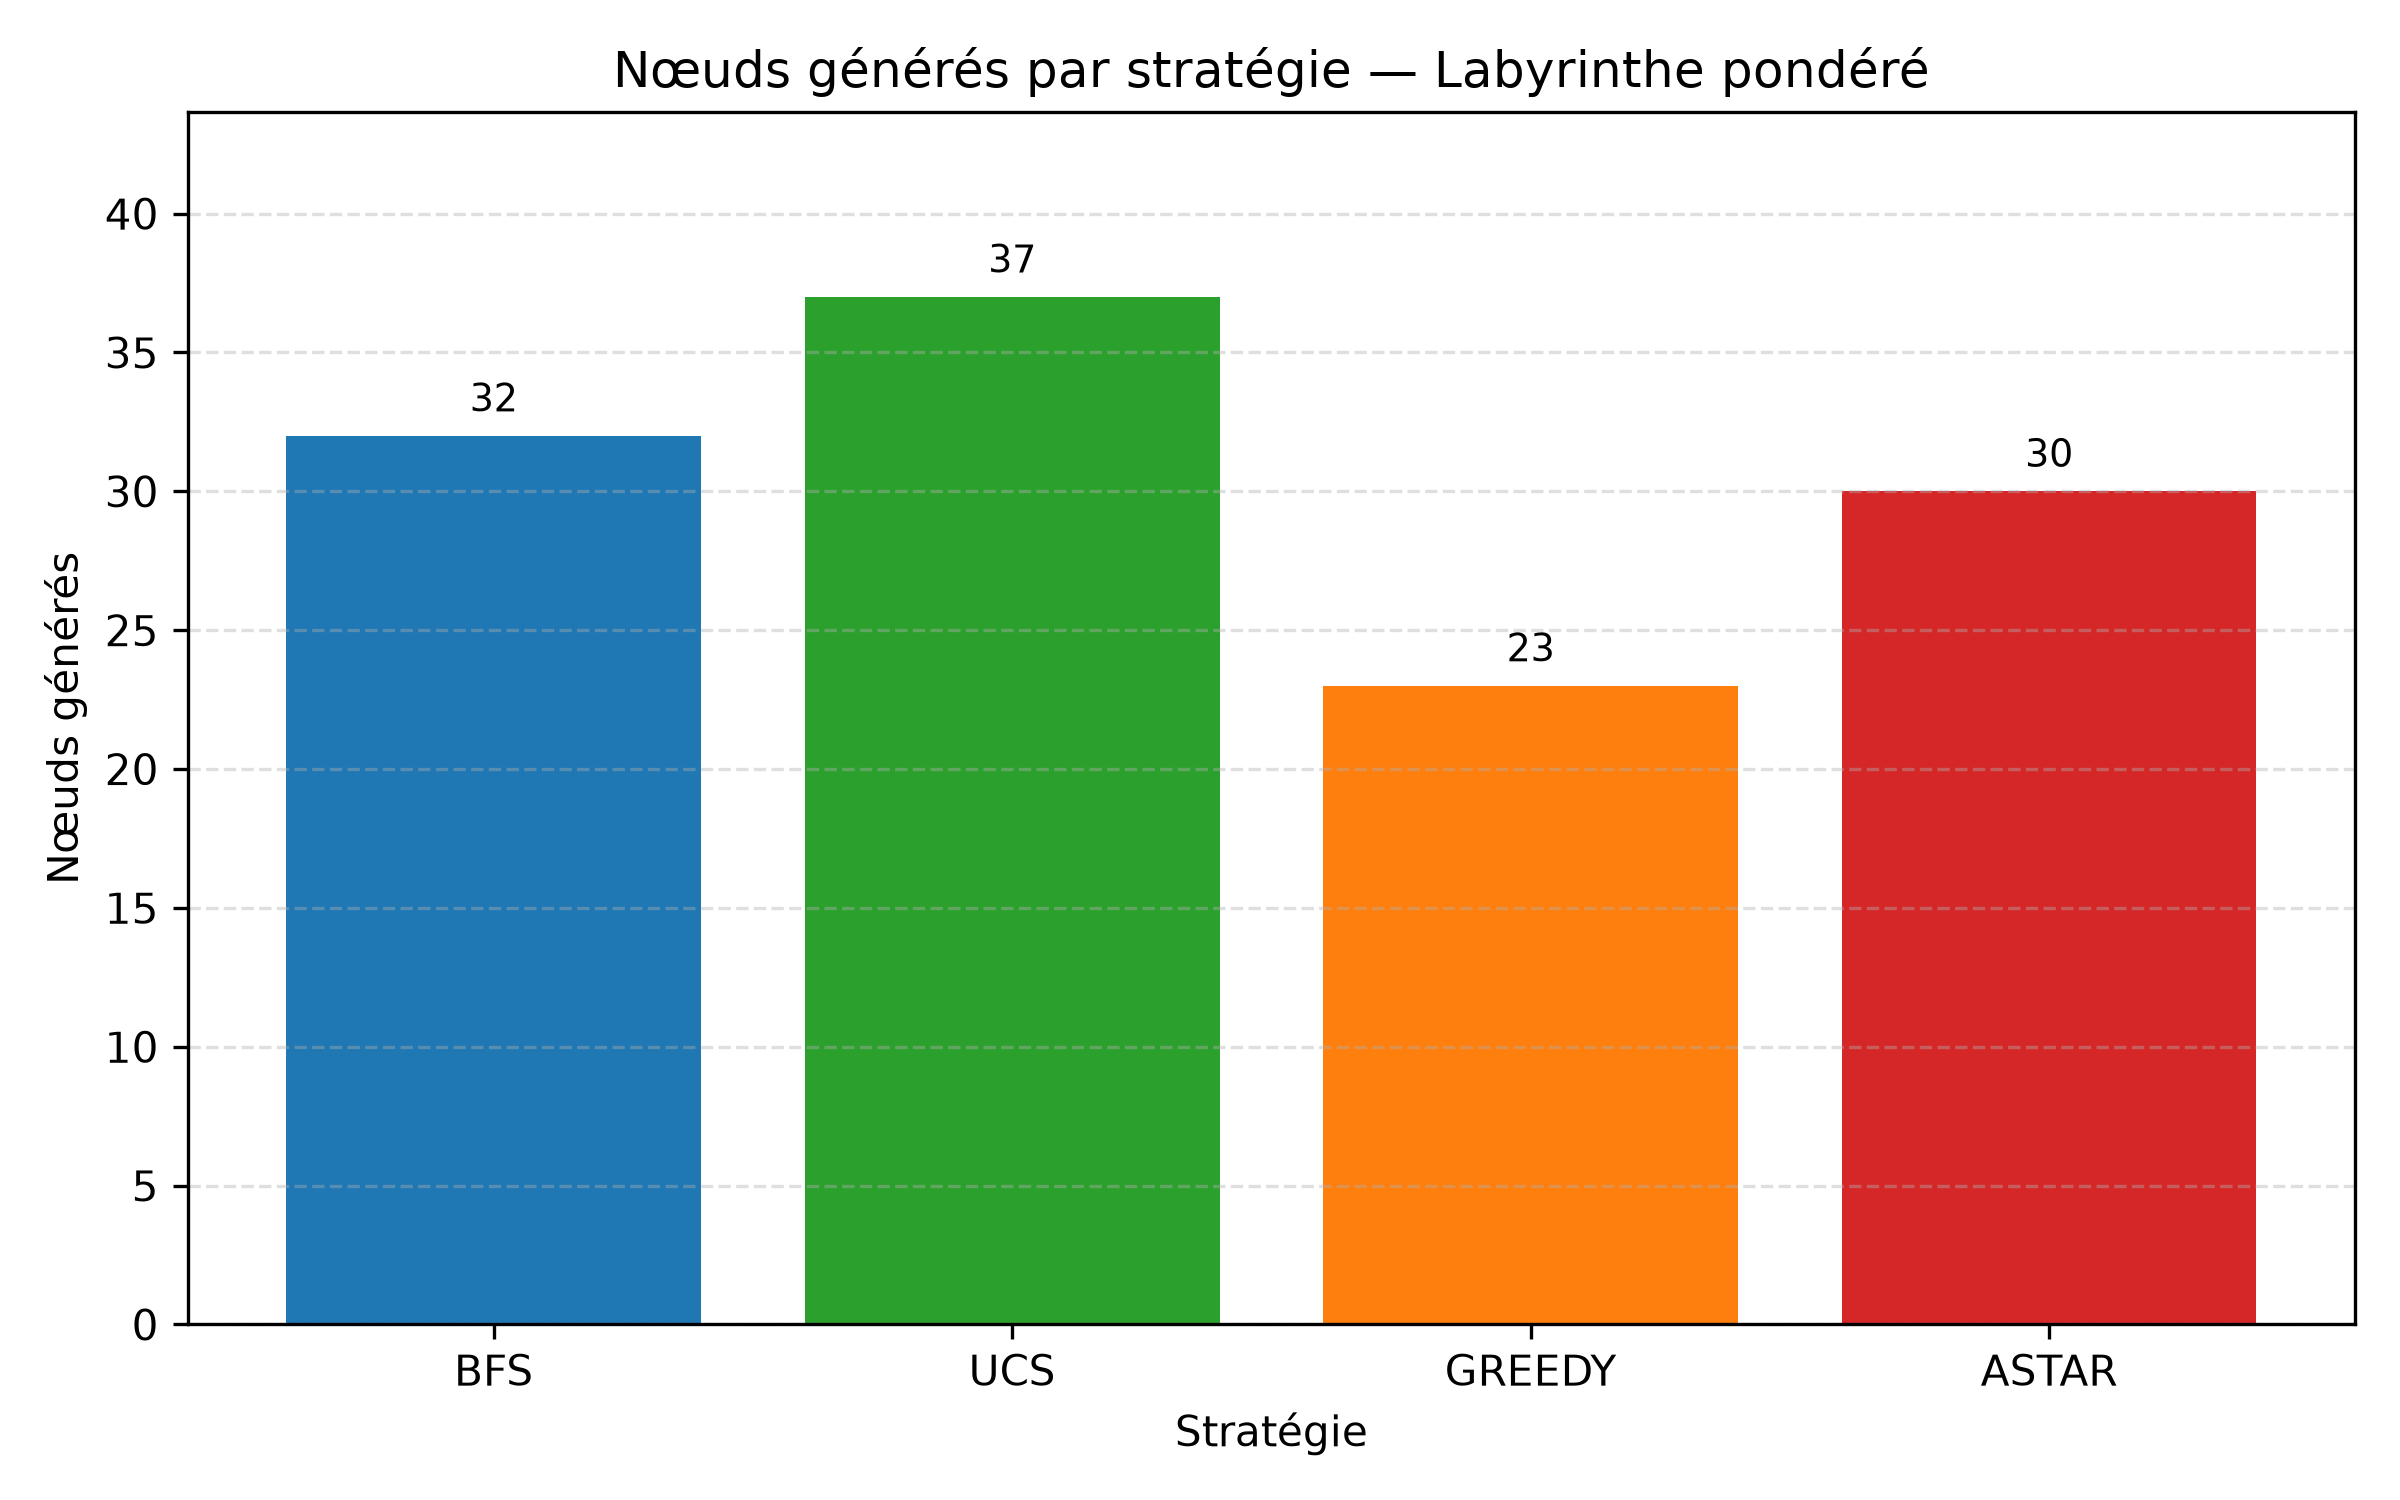
\includegraphics[width=0.78\textwidth]{figures/strategies_noeuds.png}
\caption{Noeuds générés par stratégie sur le labyrinthe pondéré en
\GraphSearch{}.}
\label{fig:strategies-noeuds}
\end{figure}

\begin{figure}[H]
\centering
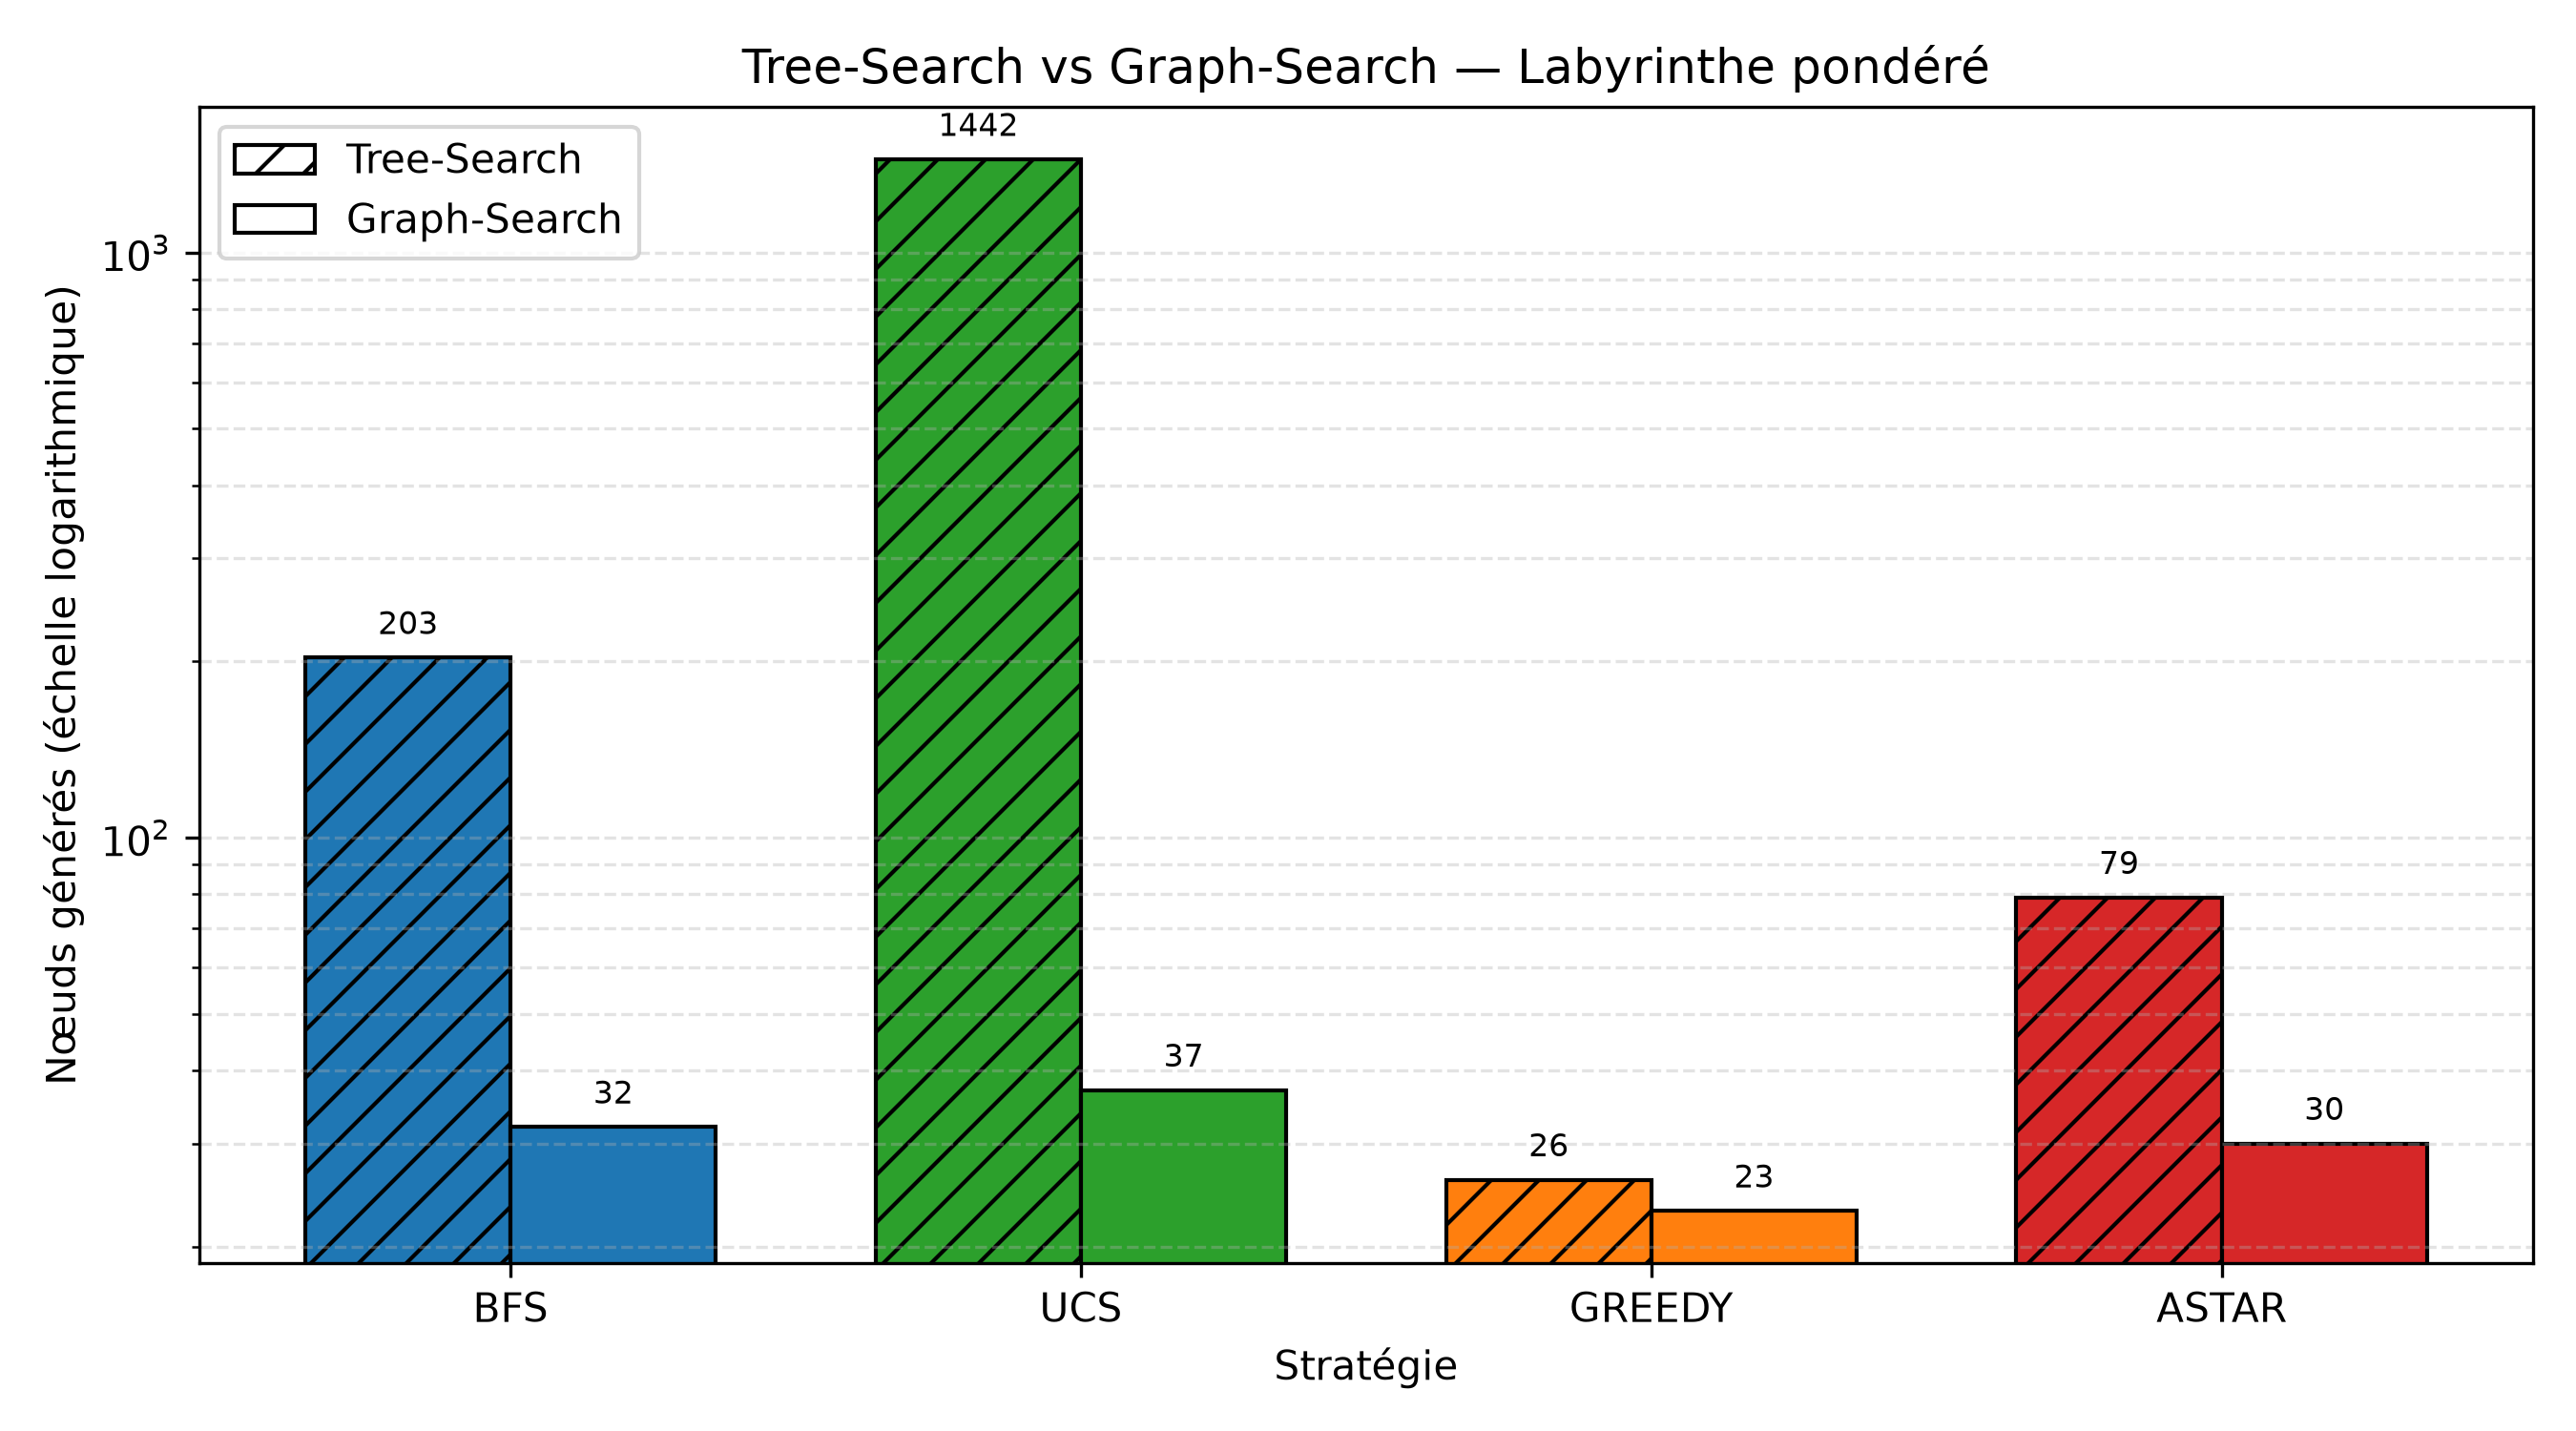
\includegraphics[width=0.82\textwidth]{figures/tree_vs_graph.png}
\caption{Noeuds générés en recherche arbre et graphe sur le labyrinthe
pondéré. L'axe vertical est logarithmique.}
\label{fig:tree-vs-graph}
\end{figure}

Sur ce labyrinthe, \GraphSearch{} réduit les noeuds expansés de 84,7\,\% pour
\BFS{} et de 97,5\,\% pour \UCS{}, par rapport à \TreeSearch{}. Pour Greedy, la
réduction est de 10,0\,\%, et pour \AStar{}, de 61,3\,\%. Le résultat dépend de
l'instance : sur le labyrinthe simple, les réductions correspondantes sont
respectivement de 50,0\,\%, 71,4\,\%, 0\,\% et 0\,\%.

\begin{figure}[H]
\centering
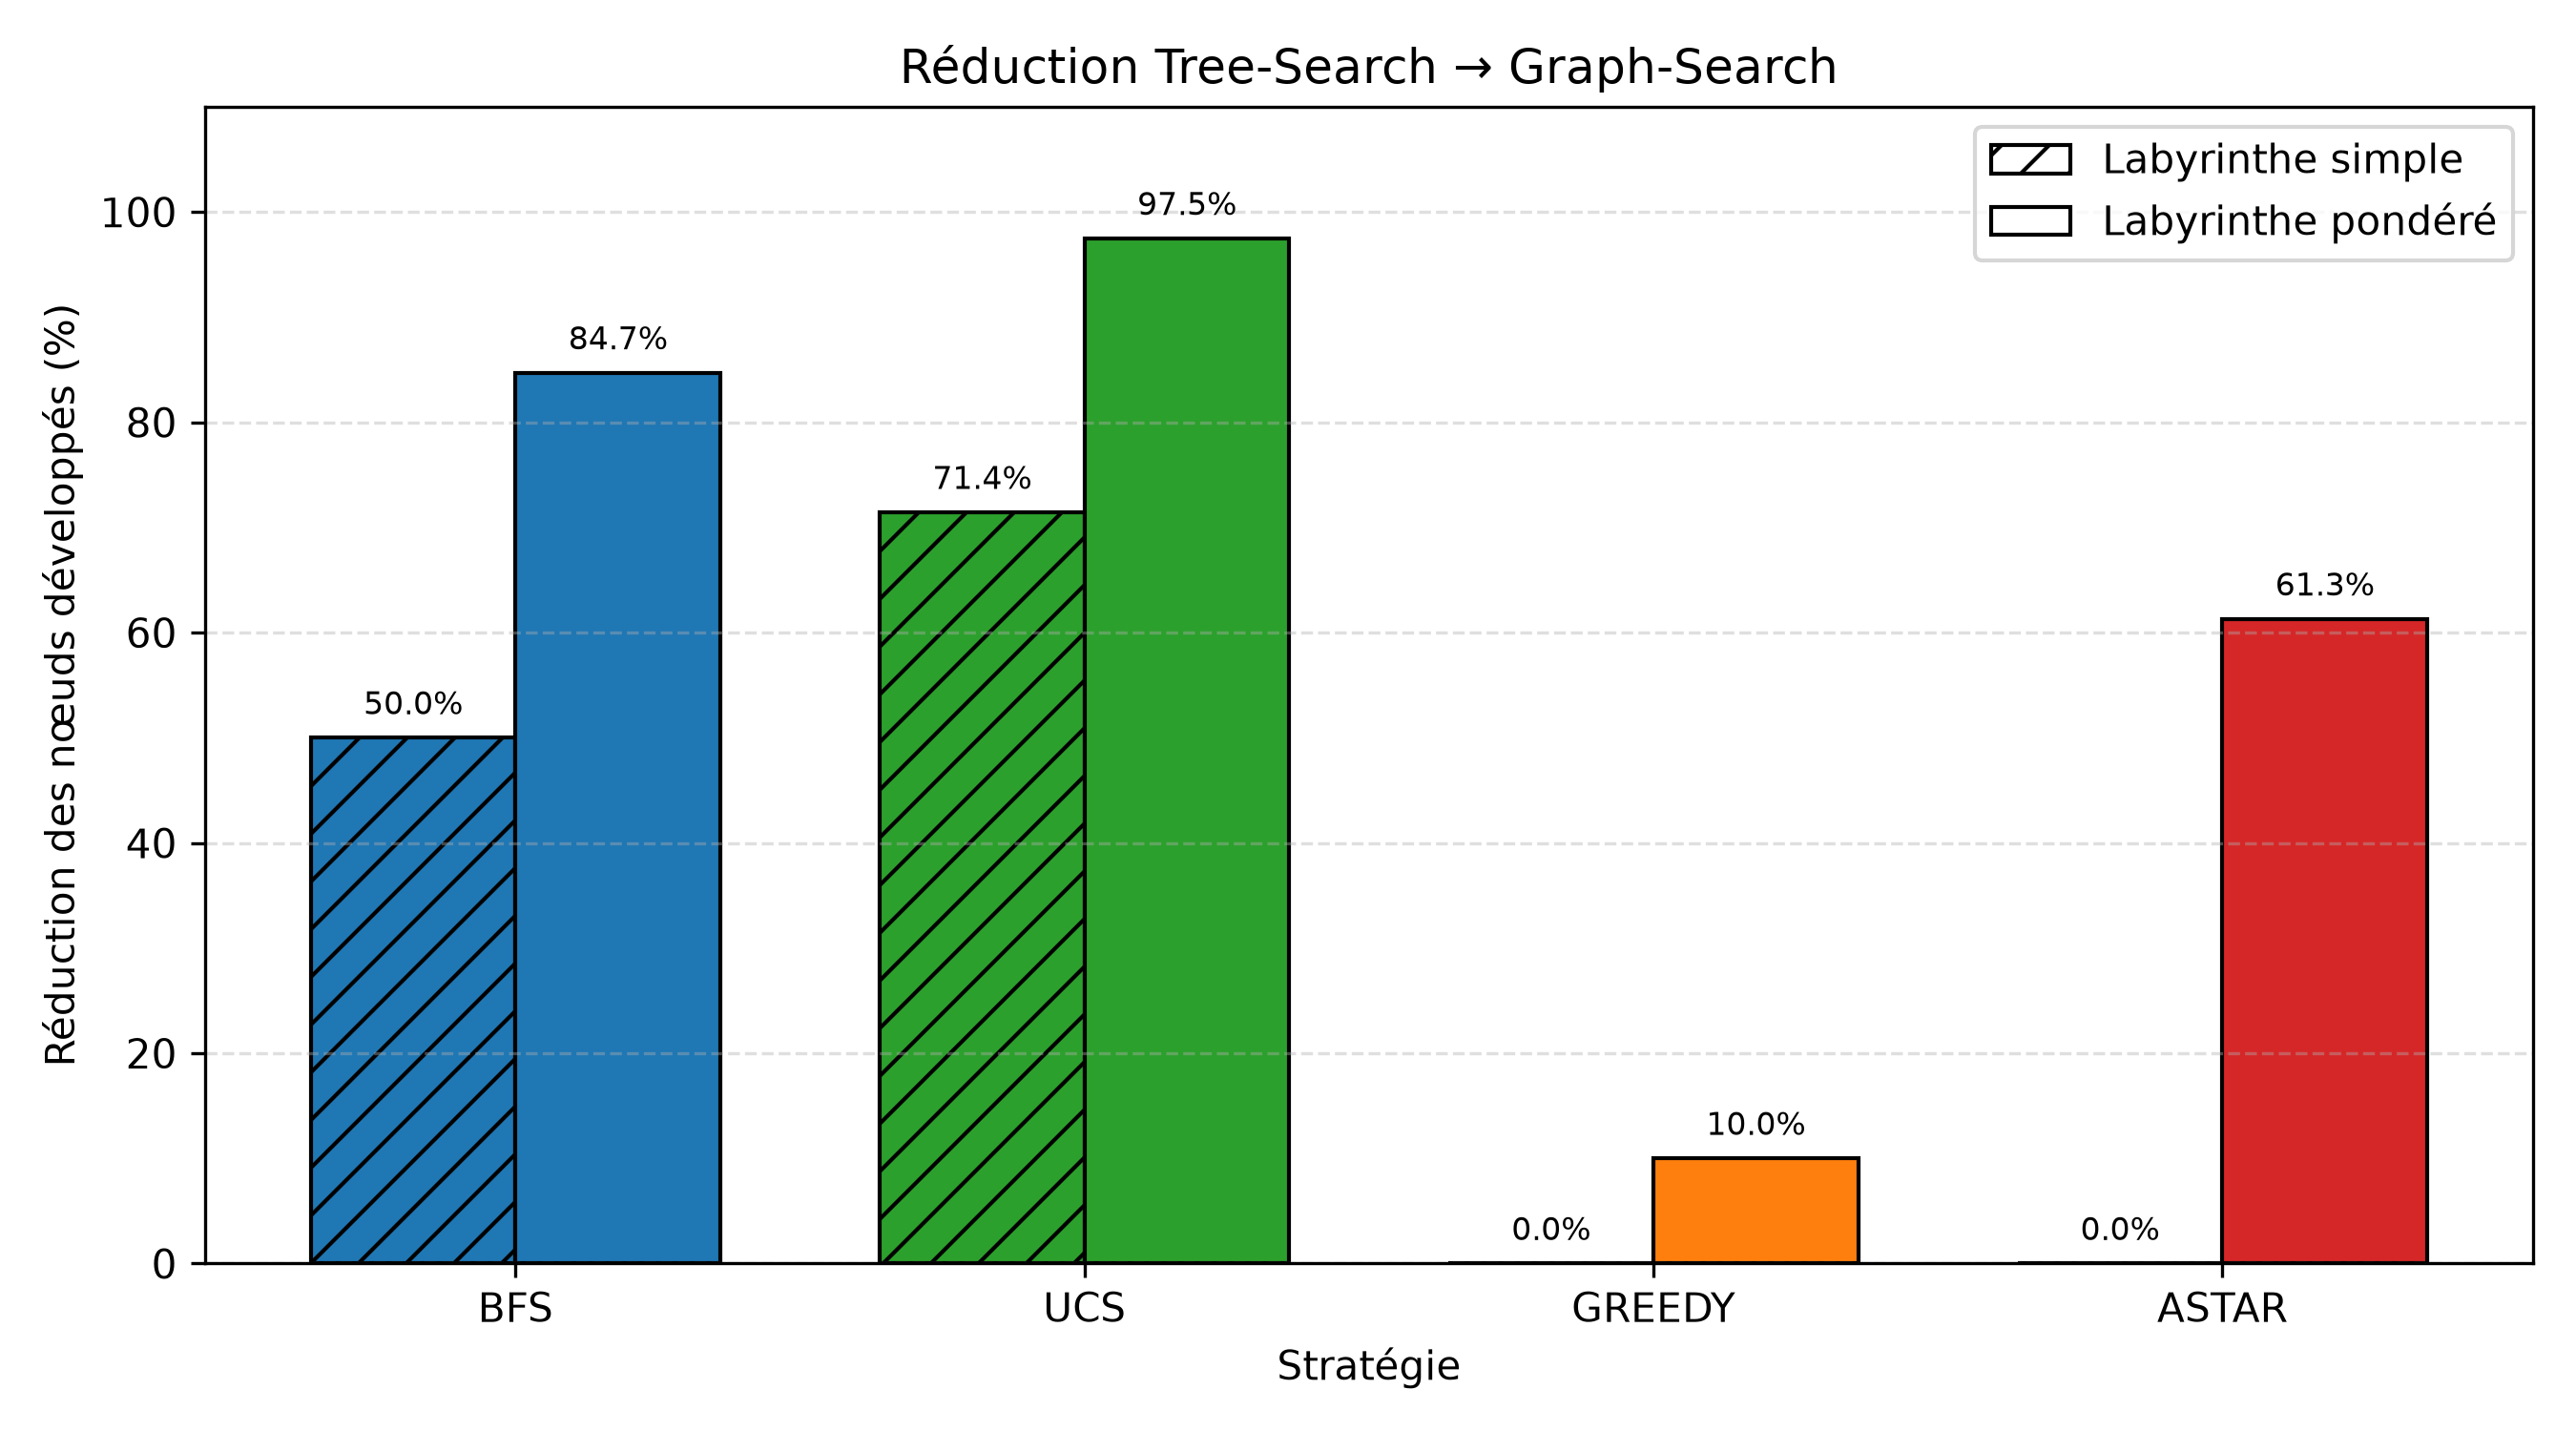
\includegraphics[width=0.78\textwidth]{figures/tree_graph_reduction.png}
\caption{Réduction du nombre de noeuds expansés obtenue avec
\GraphSearch{} sur les deux labyrinthes.}
\label{fig:tree-graph-reduction}
\end{figure}

\subsection{Navigation routière}

Pour le trajet Gatineau--Baie-Comeau, \UCS{} et \AStar{} obtiennent le coût
minimal mesuré de 881,9\,km. \BFS{} et Greedy retournent un trajet de
912,7\,km, de profondeur plus faible. Greedy est le moins expansif avec 6
noeuds, mais ne produit pas le trajet de coût minimal dans cette expérience.

\begin{table}[H]
\centering
\caption{Résultats de navigation de Gatineau à Baie-Comeau en
\GraphSearch{}.}
\label{tab:navigation}
\small
\begin{tabular}{lrrrrrr}
\toprule
\textbf{Stratégie} & \textbf{Coût (km)} & \textbf{Profondeur} &
\textbf{Gén.} & \textbf{Exp.} & \textbf{OPEN max.} & \textbf{Temps (s)} \\
\midrule
BFS & 912,7 & 6 & 69 & 23 & 7 & 0,000081 \\
UCS & 881,9 & 9 & 74 & 25 & 6 & 0,000078 \\
Greedy & 912,7 & 6 & 24 & 6 & 10 & 0,000057 \\
A* & 881,9 & 9 & 48 & 15 & 9 & 0,000112 \\
\bottomrule
\end{tabular}
\end{table}

\begin{figure}[H]
\centering
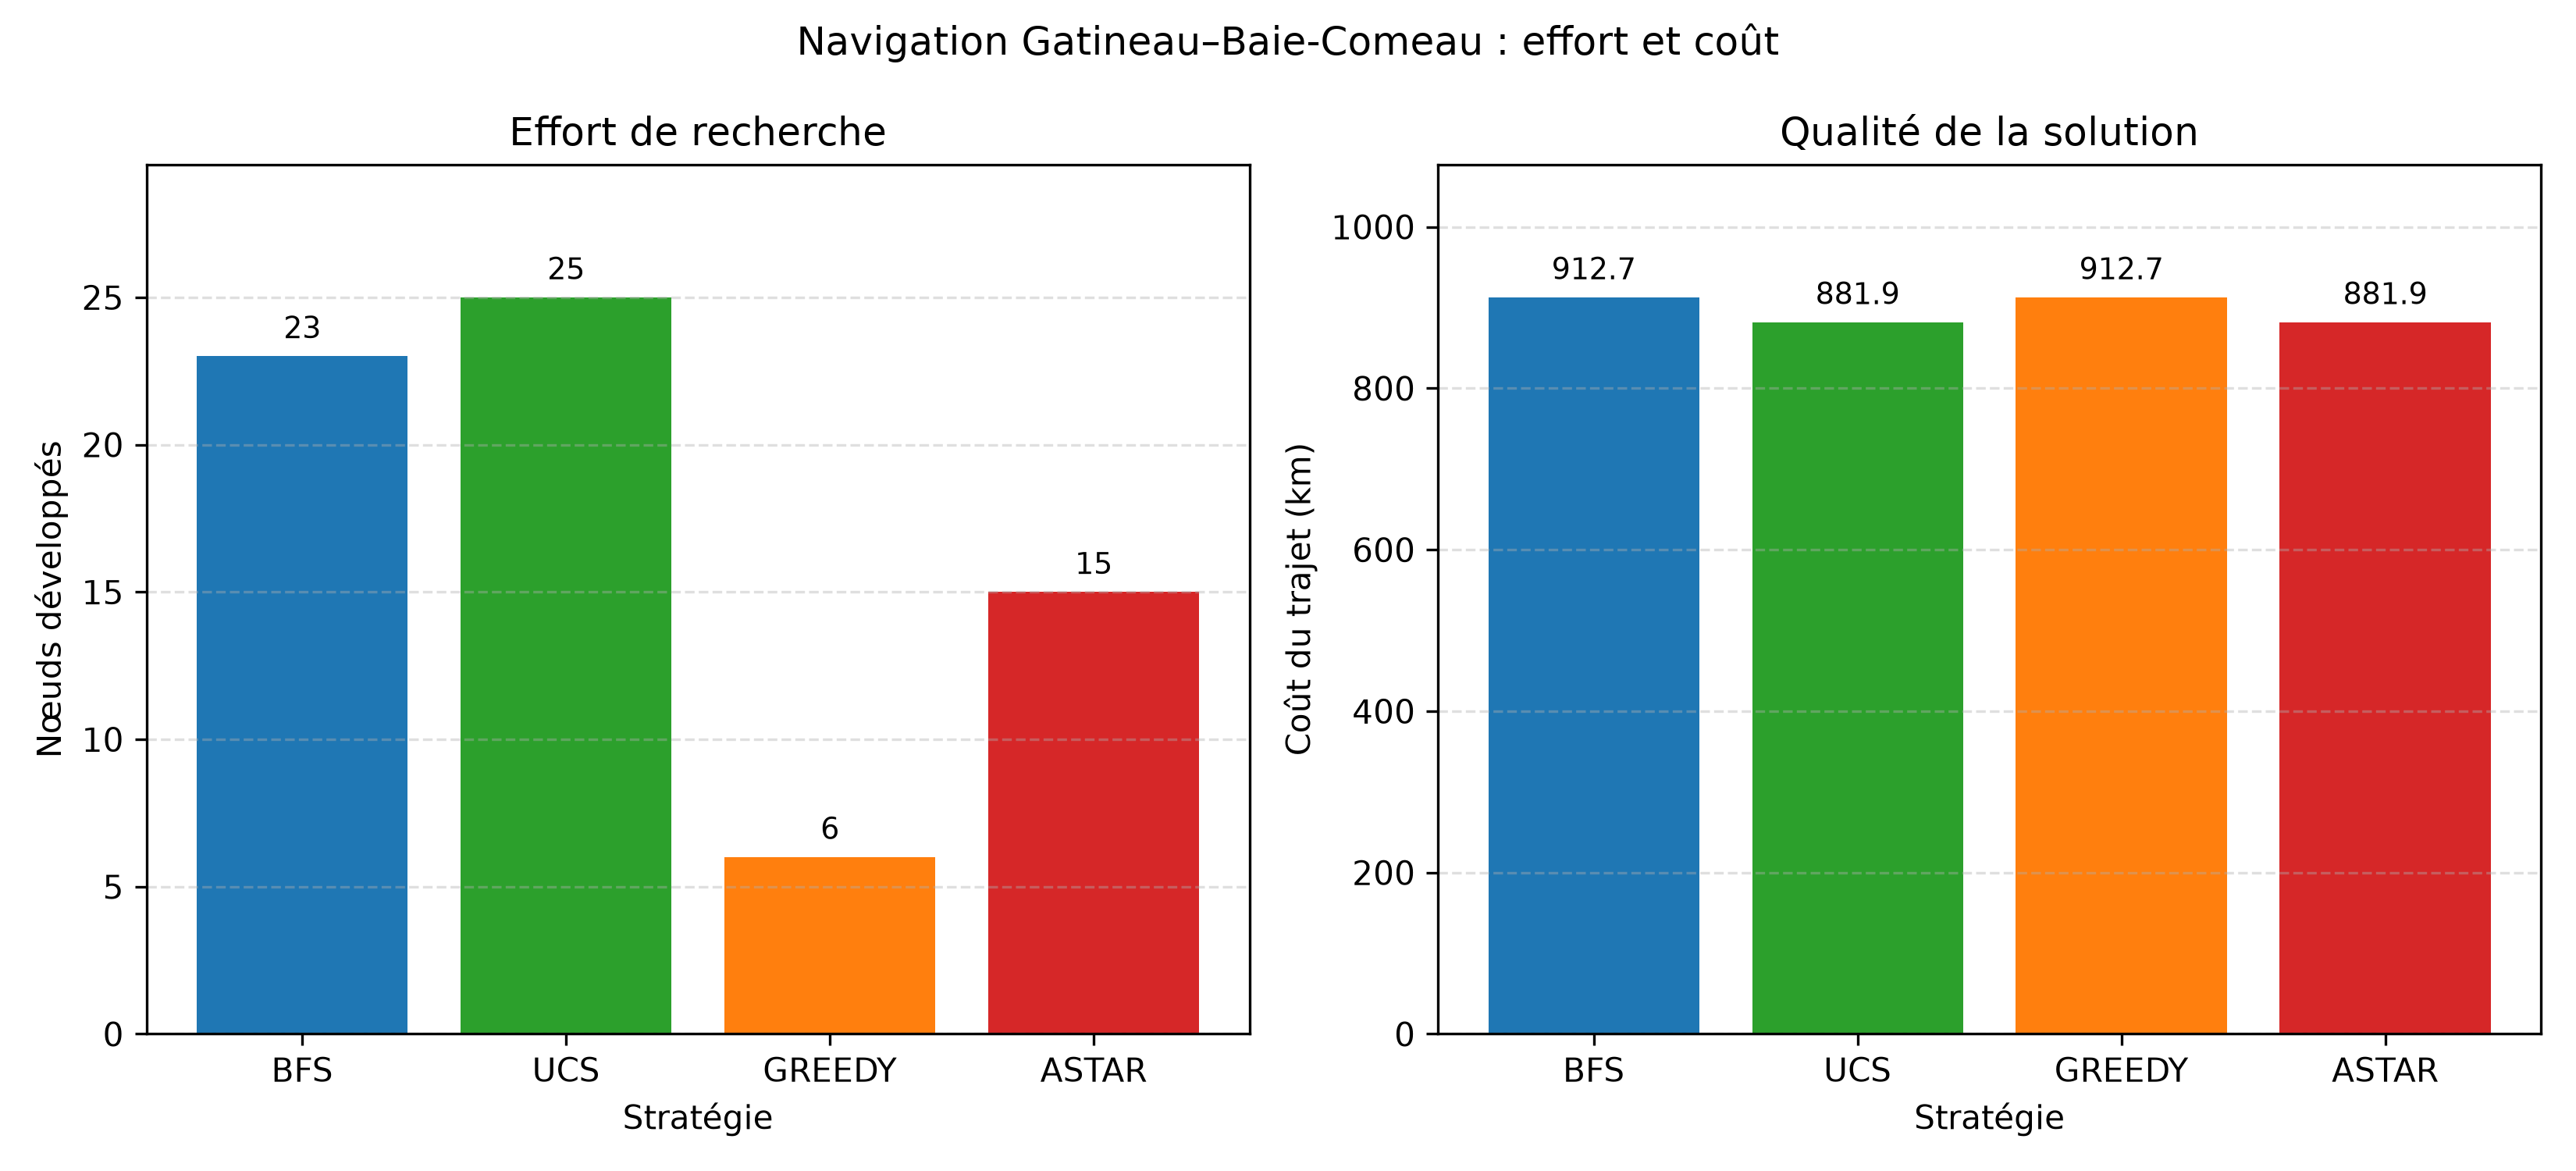
\includegraphics[width=0.92\textwidth]{figures/navigation_strategies.png}
\caption{Effort de recherche et coût de la solution pour le trajet
Gatineau--Baie-Comeau.}
\label{fig:navigation-strategies}
\end{figure}

\subsection{Stratégies sur le 8-Puzzle moyen}

\BFS{}, \UCS{} et \AStar{} trouvent une solution optimale de 28 coups dans
cette instance; \AStar{} développe 1\,440 noeuds contre 171\,028 pour \BFS{}.
Greedy ne développe que 385 noeuds, mais sa solution comporte 48 coups. Ce
résultat illustre le compromis entre l'effort de recherche et la qualité de
solution.

\begin{table}[H]
\centering
\caption{Comparaison des stratégies sur le 8-Puzzle moyen en
\GraphSearch{}.}
\label{tab:npuzzle-strategies}
\small
\begin{tabular}{lrrrrrr}
\toprule
\textbf{Stratégie} & \textbf{Coût} & \textbf{Profondeur} &
\textbf{Gén.} & \textbf{Exp.} & \textbf{OPEN max.} & \textbf{Temps (s)} \\
\midrule
BFS & 28 & 28 & 455\,676 & 171\,028 & 24\,053 & 1,149463 \\
UCS & 28 & 28 & 473\,571 & 177\,134 & 24\,053 & 1,267173 \\
Greedy & 48 & 48 & 1\,052 & 385 & 218 & 0,003184 \\
A* & 28 & 28 & 3\,815 & 1\,440 & 823 & 0,014050 \\
\bottomrule
\end{tabular}
\end{table}

\begin{figure}[H]
\centering
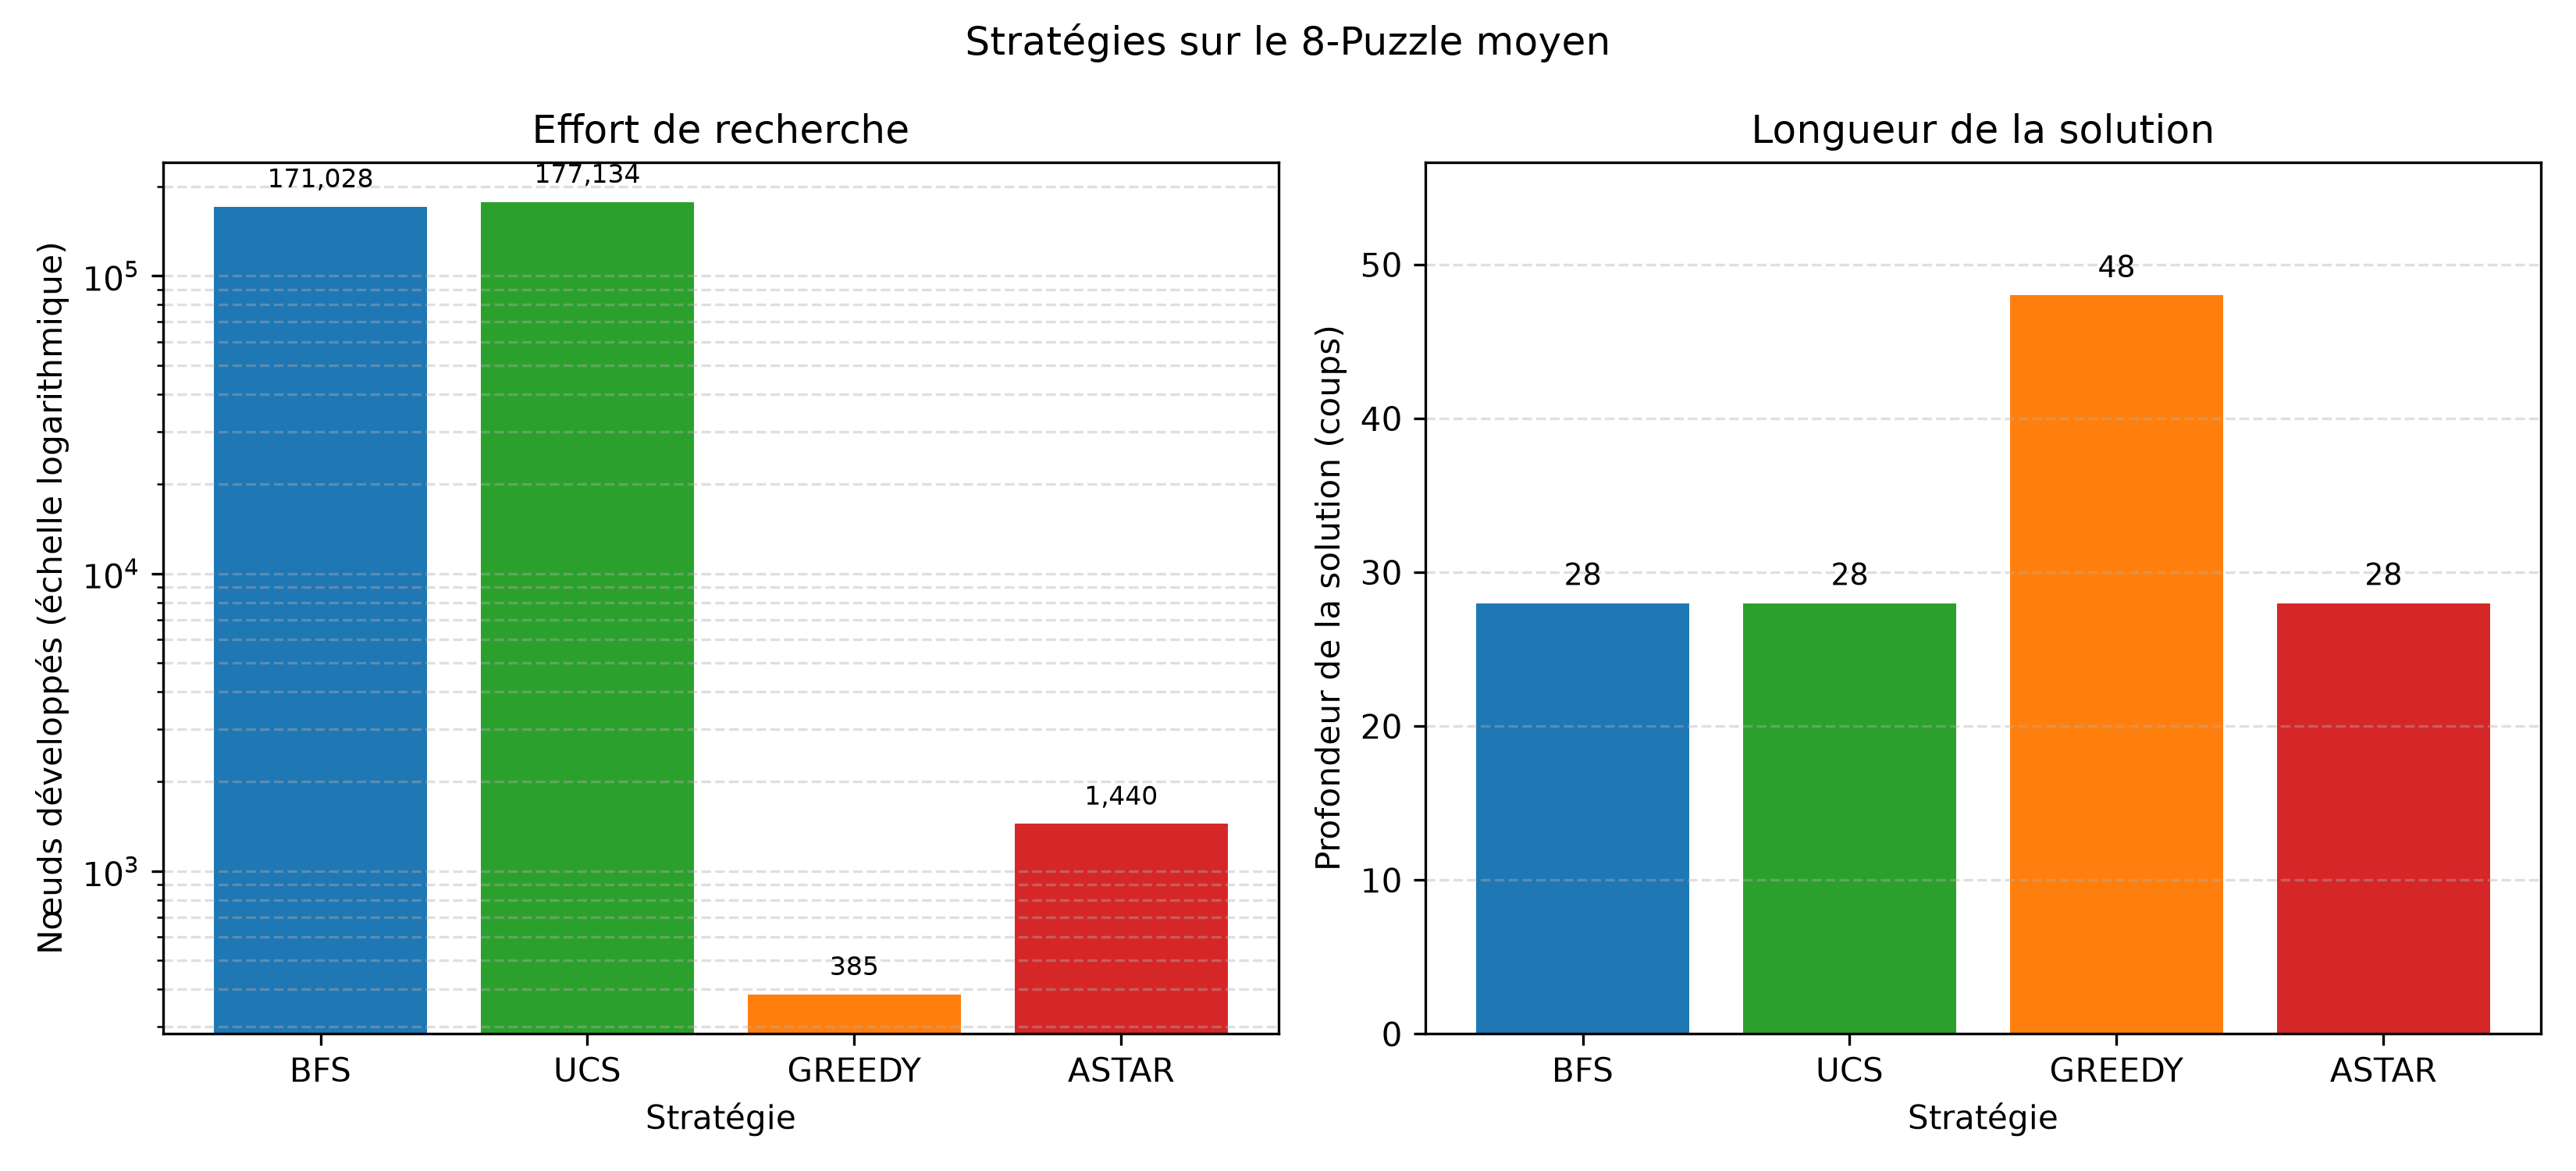
\includegraphics[width=0.92\textwidth]{figures/strategies_npuzzle.png}
\caption{Noeuds expansés et profondeur de solution selon la stratégie sur le
8-Puzzle moyen.}
\label{fig:strategies-npuzzle}
\end{figure}

\subsection{Influence des heuristiques}

Le \cref{tab:heuristique-valeurs} compare les mesures d'\AStar{} sur la même
instance moyenne de 8-Puzzle. Les trois variantes trouvent une solution de coût
28 et de profondeur 28. Manhattan réduit les noeuds expansés de 99,2\,\% par
rapport à $h=0$; l'heuristique des tuiles mal placées les réduit de 66,7\,\%.
Le temps mesuré pour Manhattan est de 0,014178\,s contre 1,388574\,s avec
$h=0$; ces temps ne proviennent que d'une exécution chacun.

\begin{table}[H]
\centering
\caption{Résultats d'\AStar{} selon l'heuristique sur le 8-Puzzle moyen.}
\label{tab:heuristique-valeurs}
\small
\begin{tabular}{lrrrrrr}
\toprule
\textbf{Heuristique} & \textbf{Coût / prof.} & \textbf{Gén.} &
\textbf{Exp.} & \textbf{OPEN max.} & \textbf{Temps (s)} &
\textbf{Réduction exp.} \\
\midrule
$h=0$ & 28 / 28 & 473\,571 & 177\,134 & 24\,053 & 1,388574 & Référence \\
Mal placées & 28 / 28 & 160\,091 & 59\,067 & 22\,060 & 0,592204 & 66,7\,\% \\
Manhattan & 28 / 28 & 3\,815 & 1\,440 & 823 & 0,014178 & 99,2\,\% \\
\bottomrule
\end{tabular}
\end{table}

\begin{figure}[H]
\centering
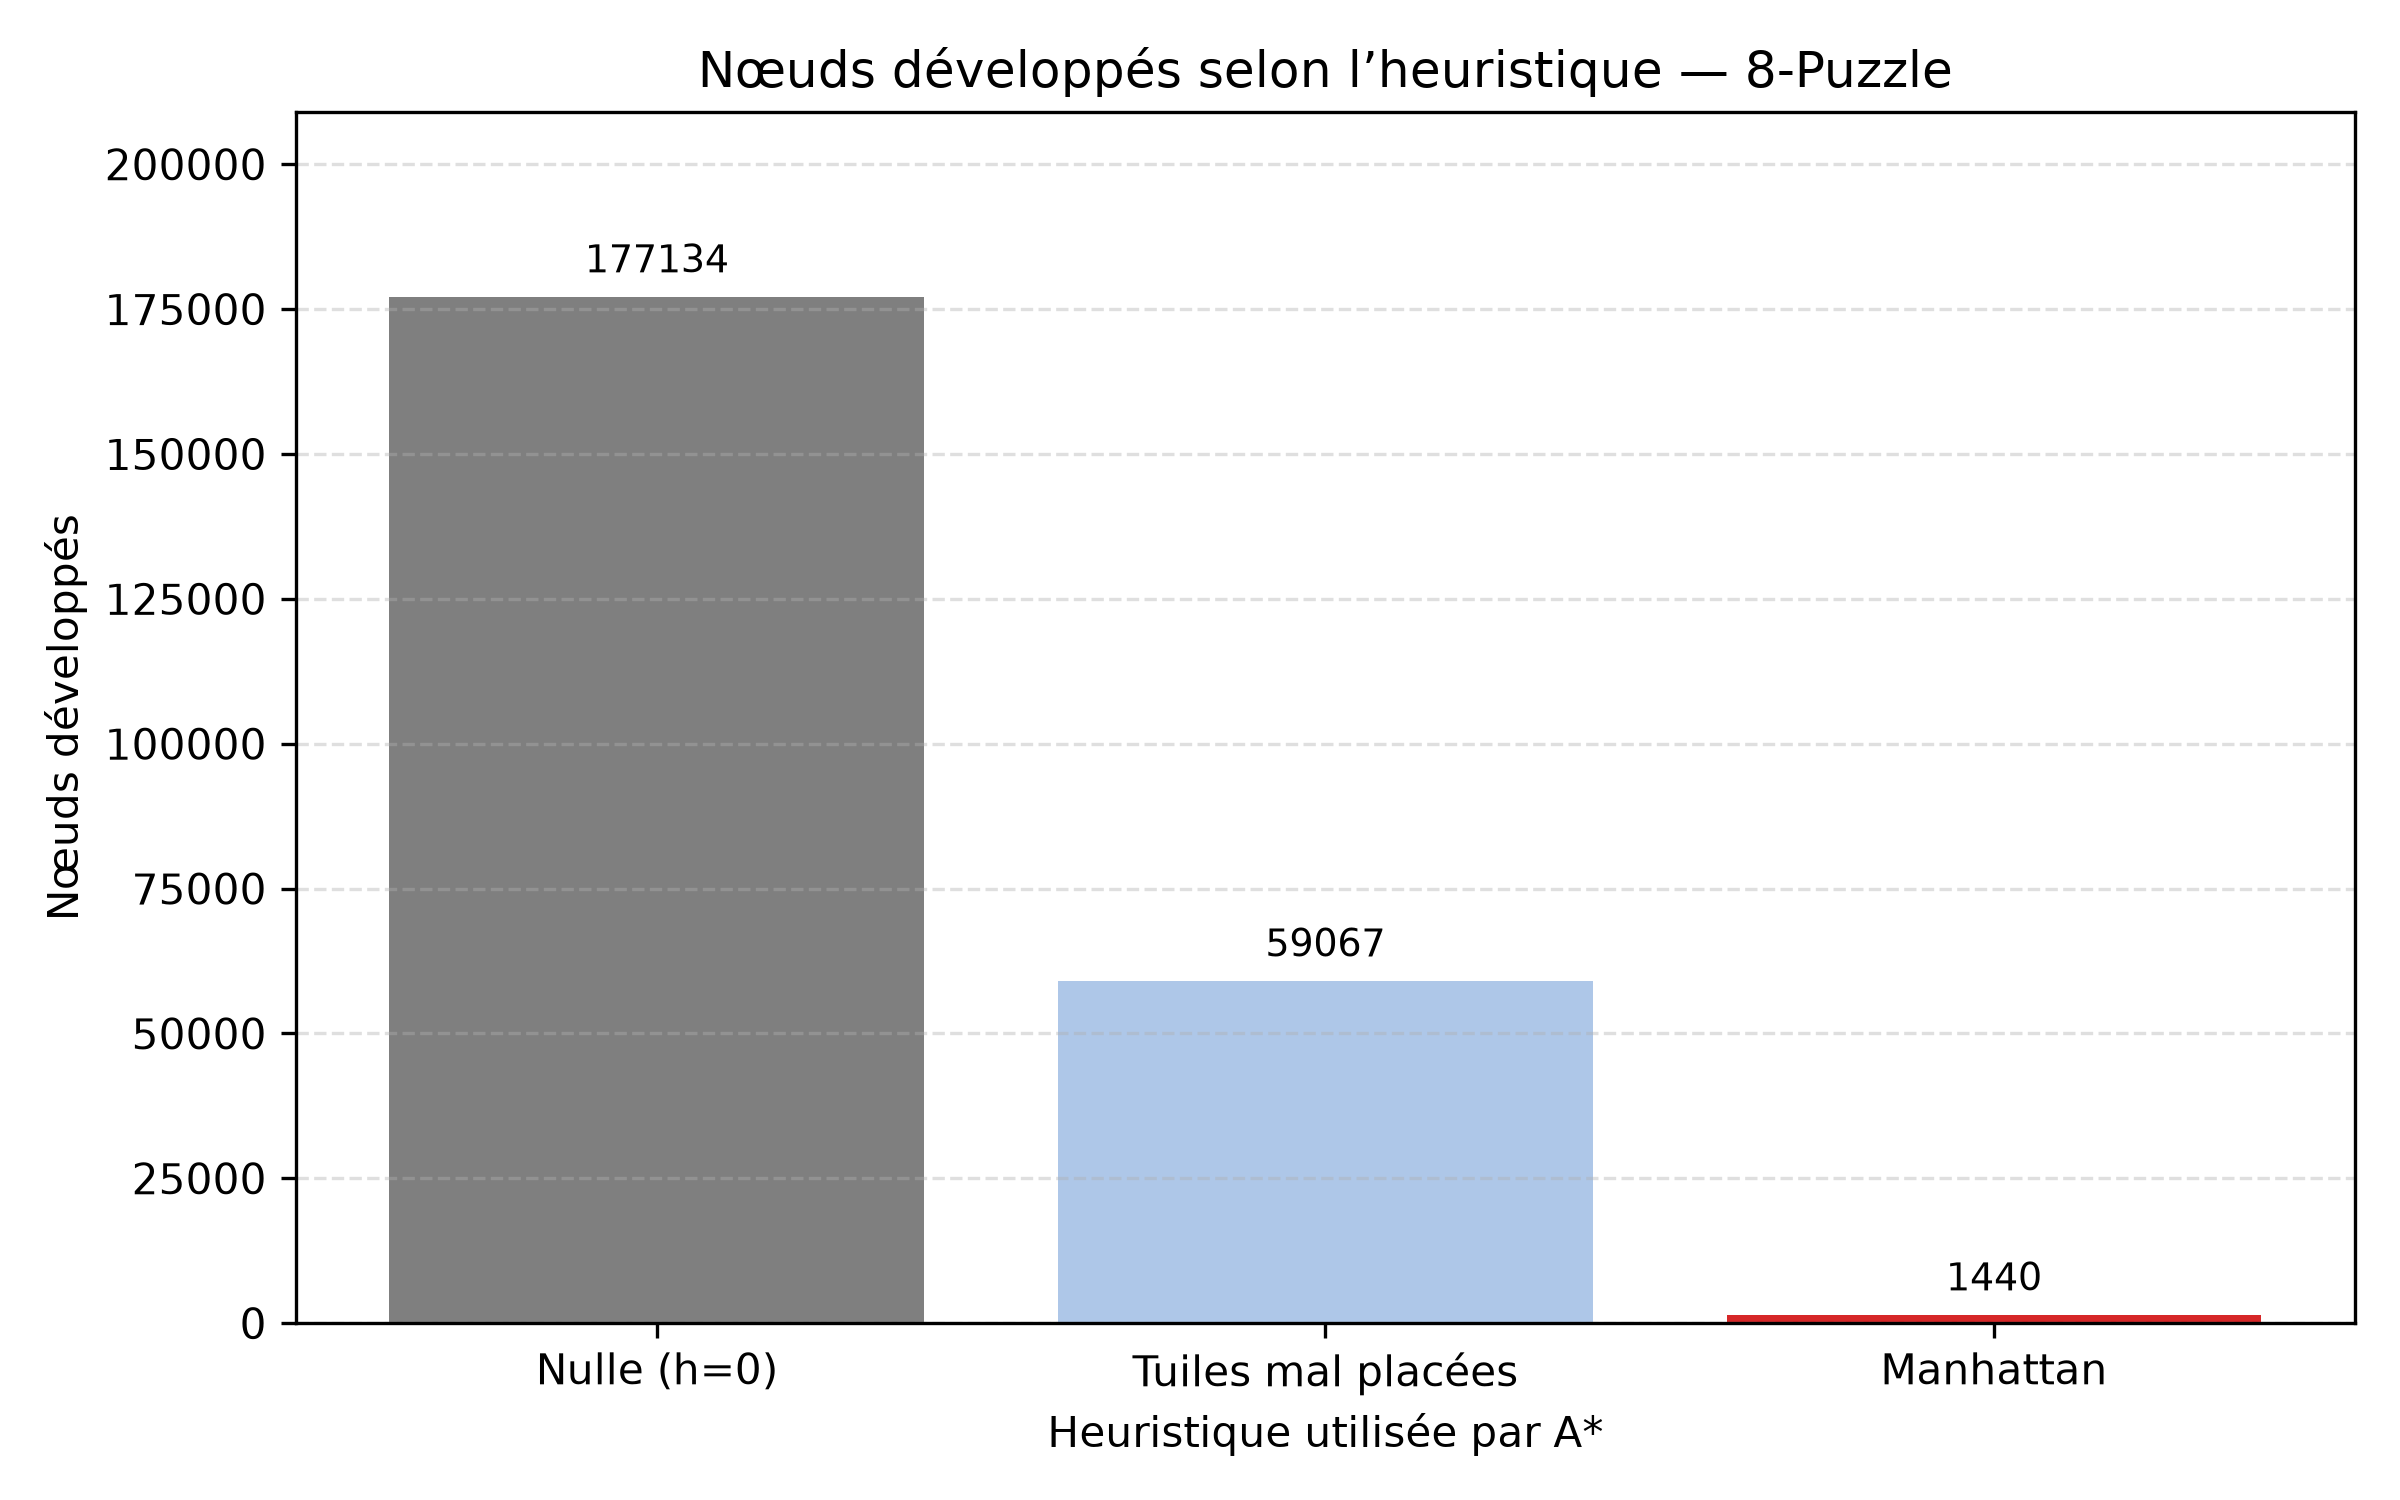
\includegraphics[width=0.82\textwidth]{figures/heuristiques_npuzzle.png}
\caption{Noeuds expansés par \AStar{} selon l'heuristique du 8-Puzzle.}
\label{fig:heuristiques-npuzzle}
\end{figure}

\begin{figure}[H]
\centering
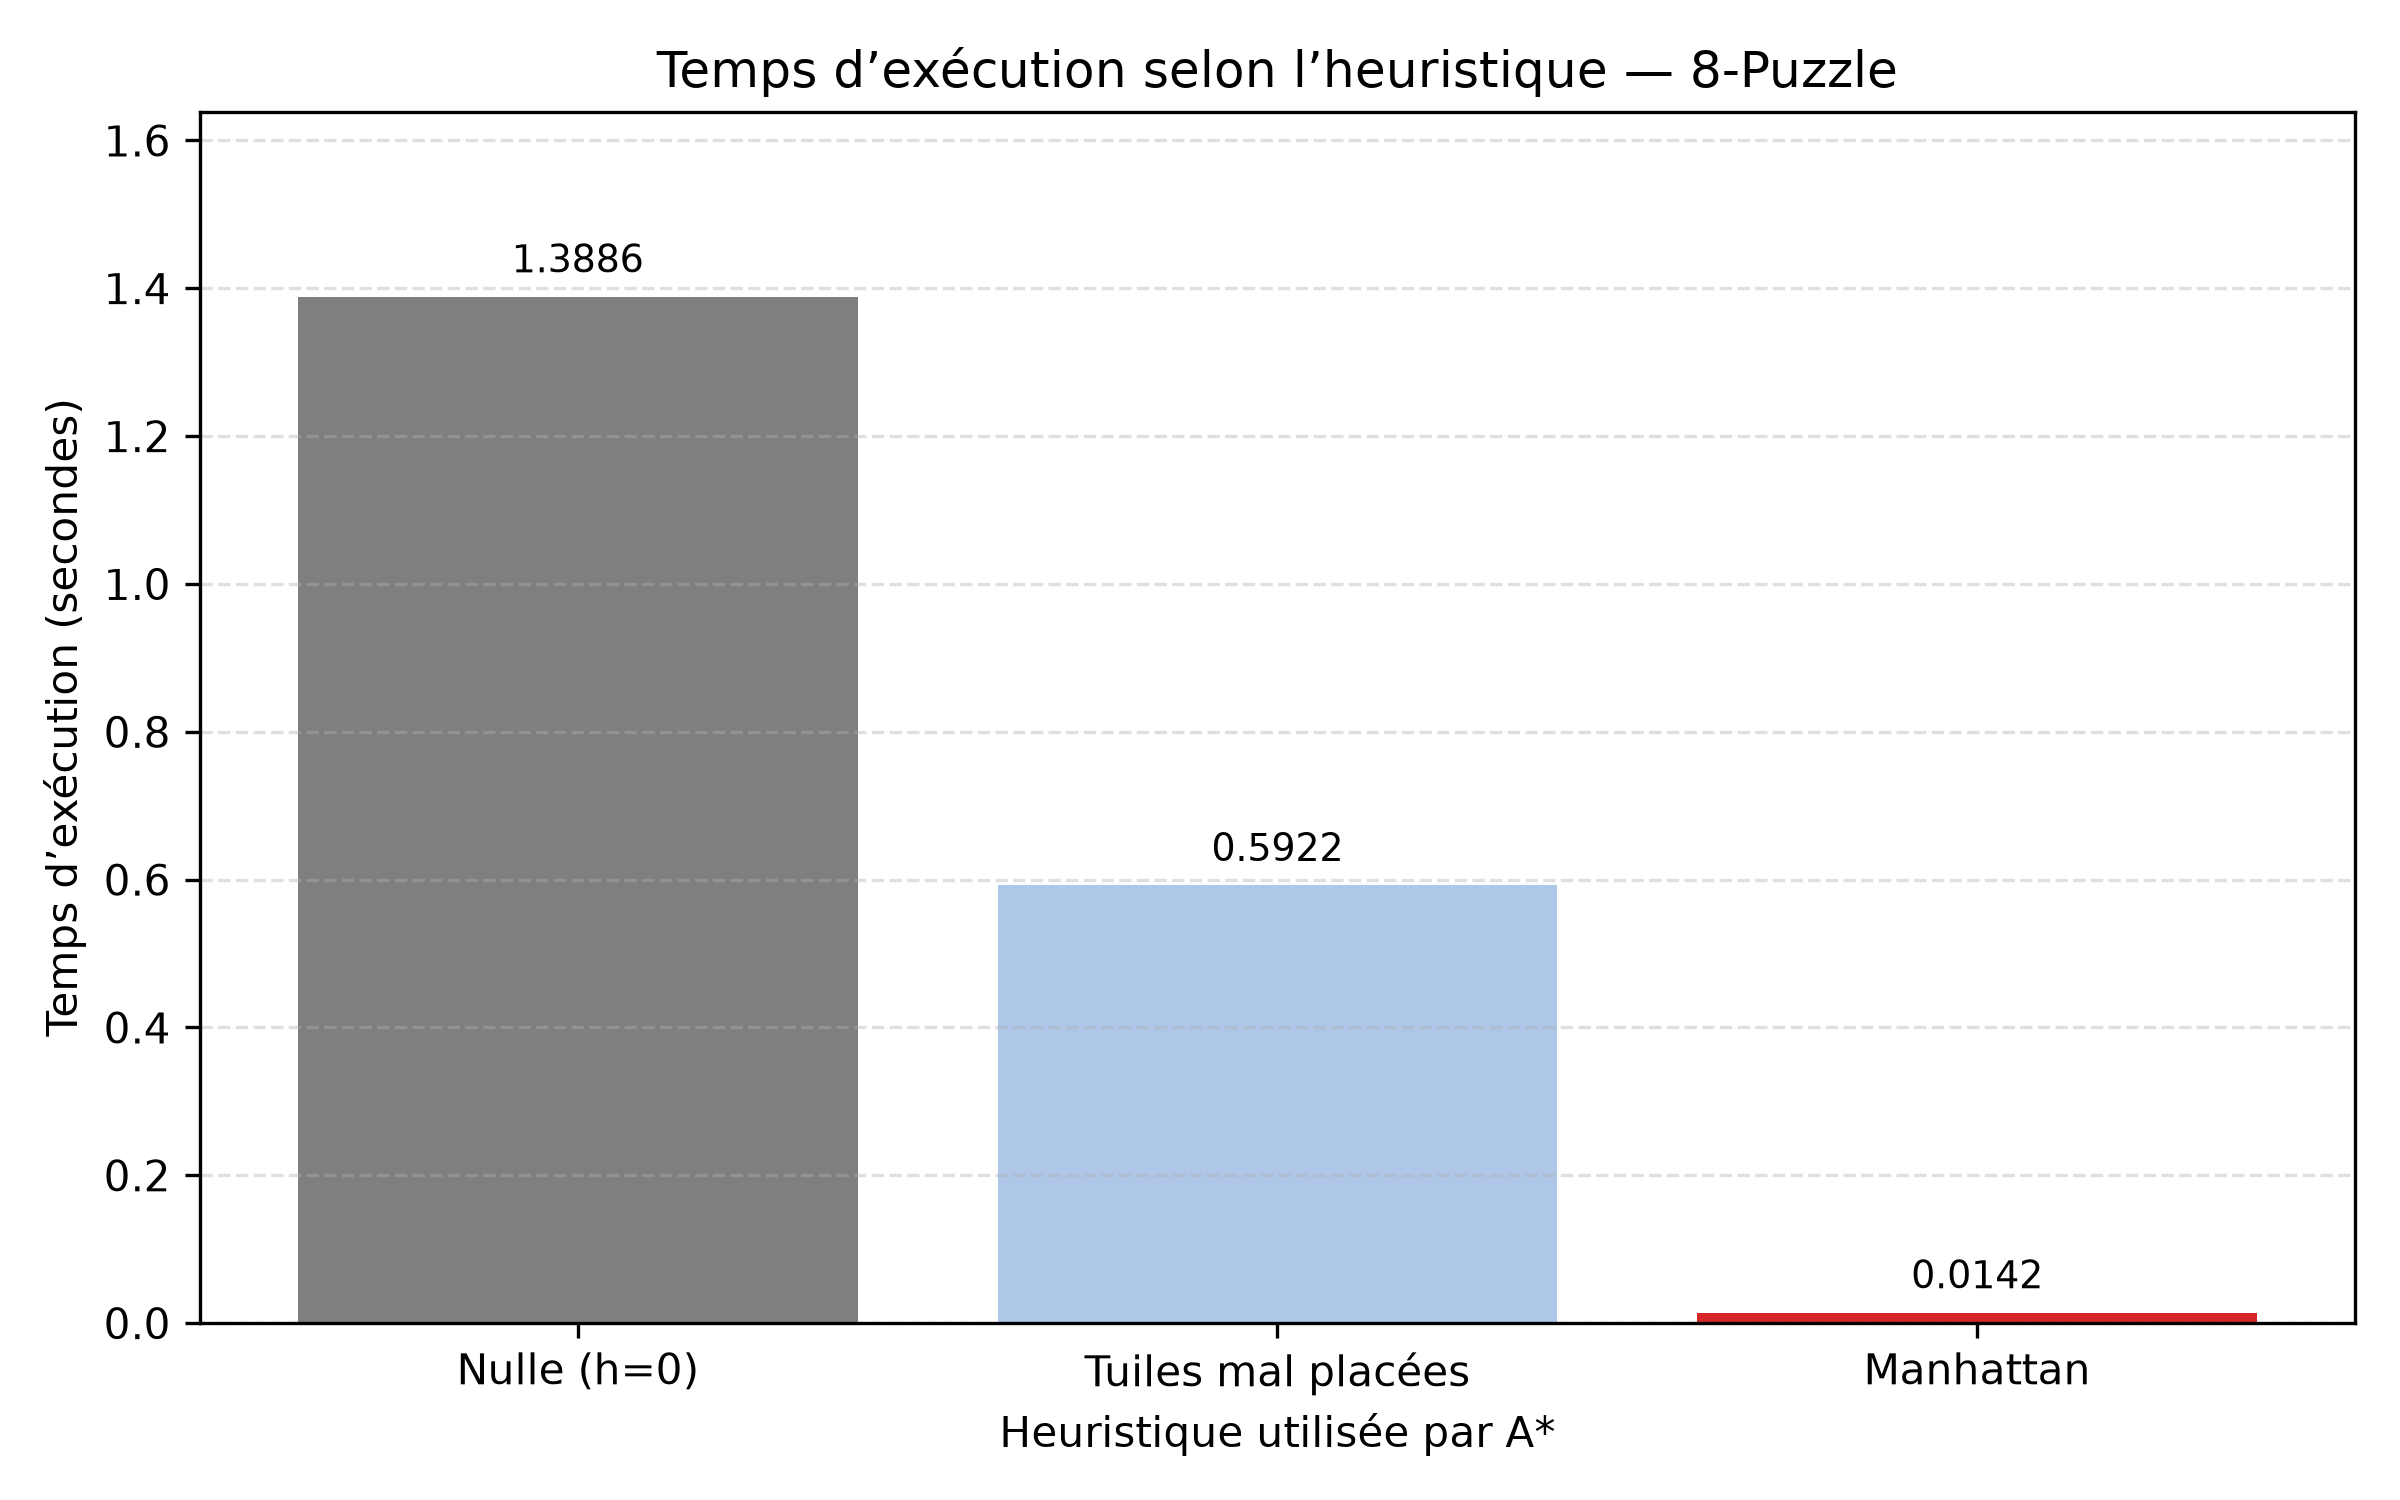
\includegraphics[width=0.82\textwidth]{figures/heuristiques_temps.png}
\caption{Temps mesuré par \AStar{} selon l'heuristique du 8-Puzzle.}
\label{fig:heuristiques-temps}
\end{figure}

\begin{figure}[H]
\centering
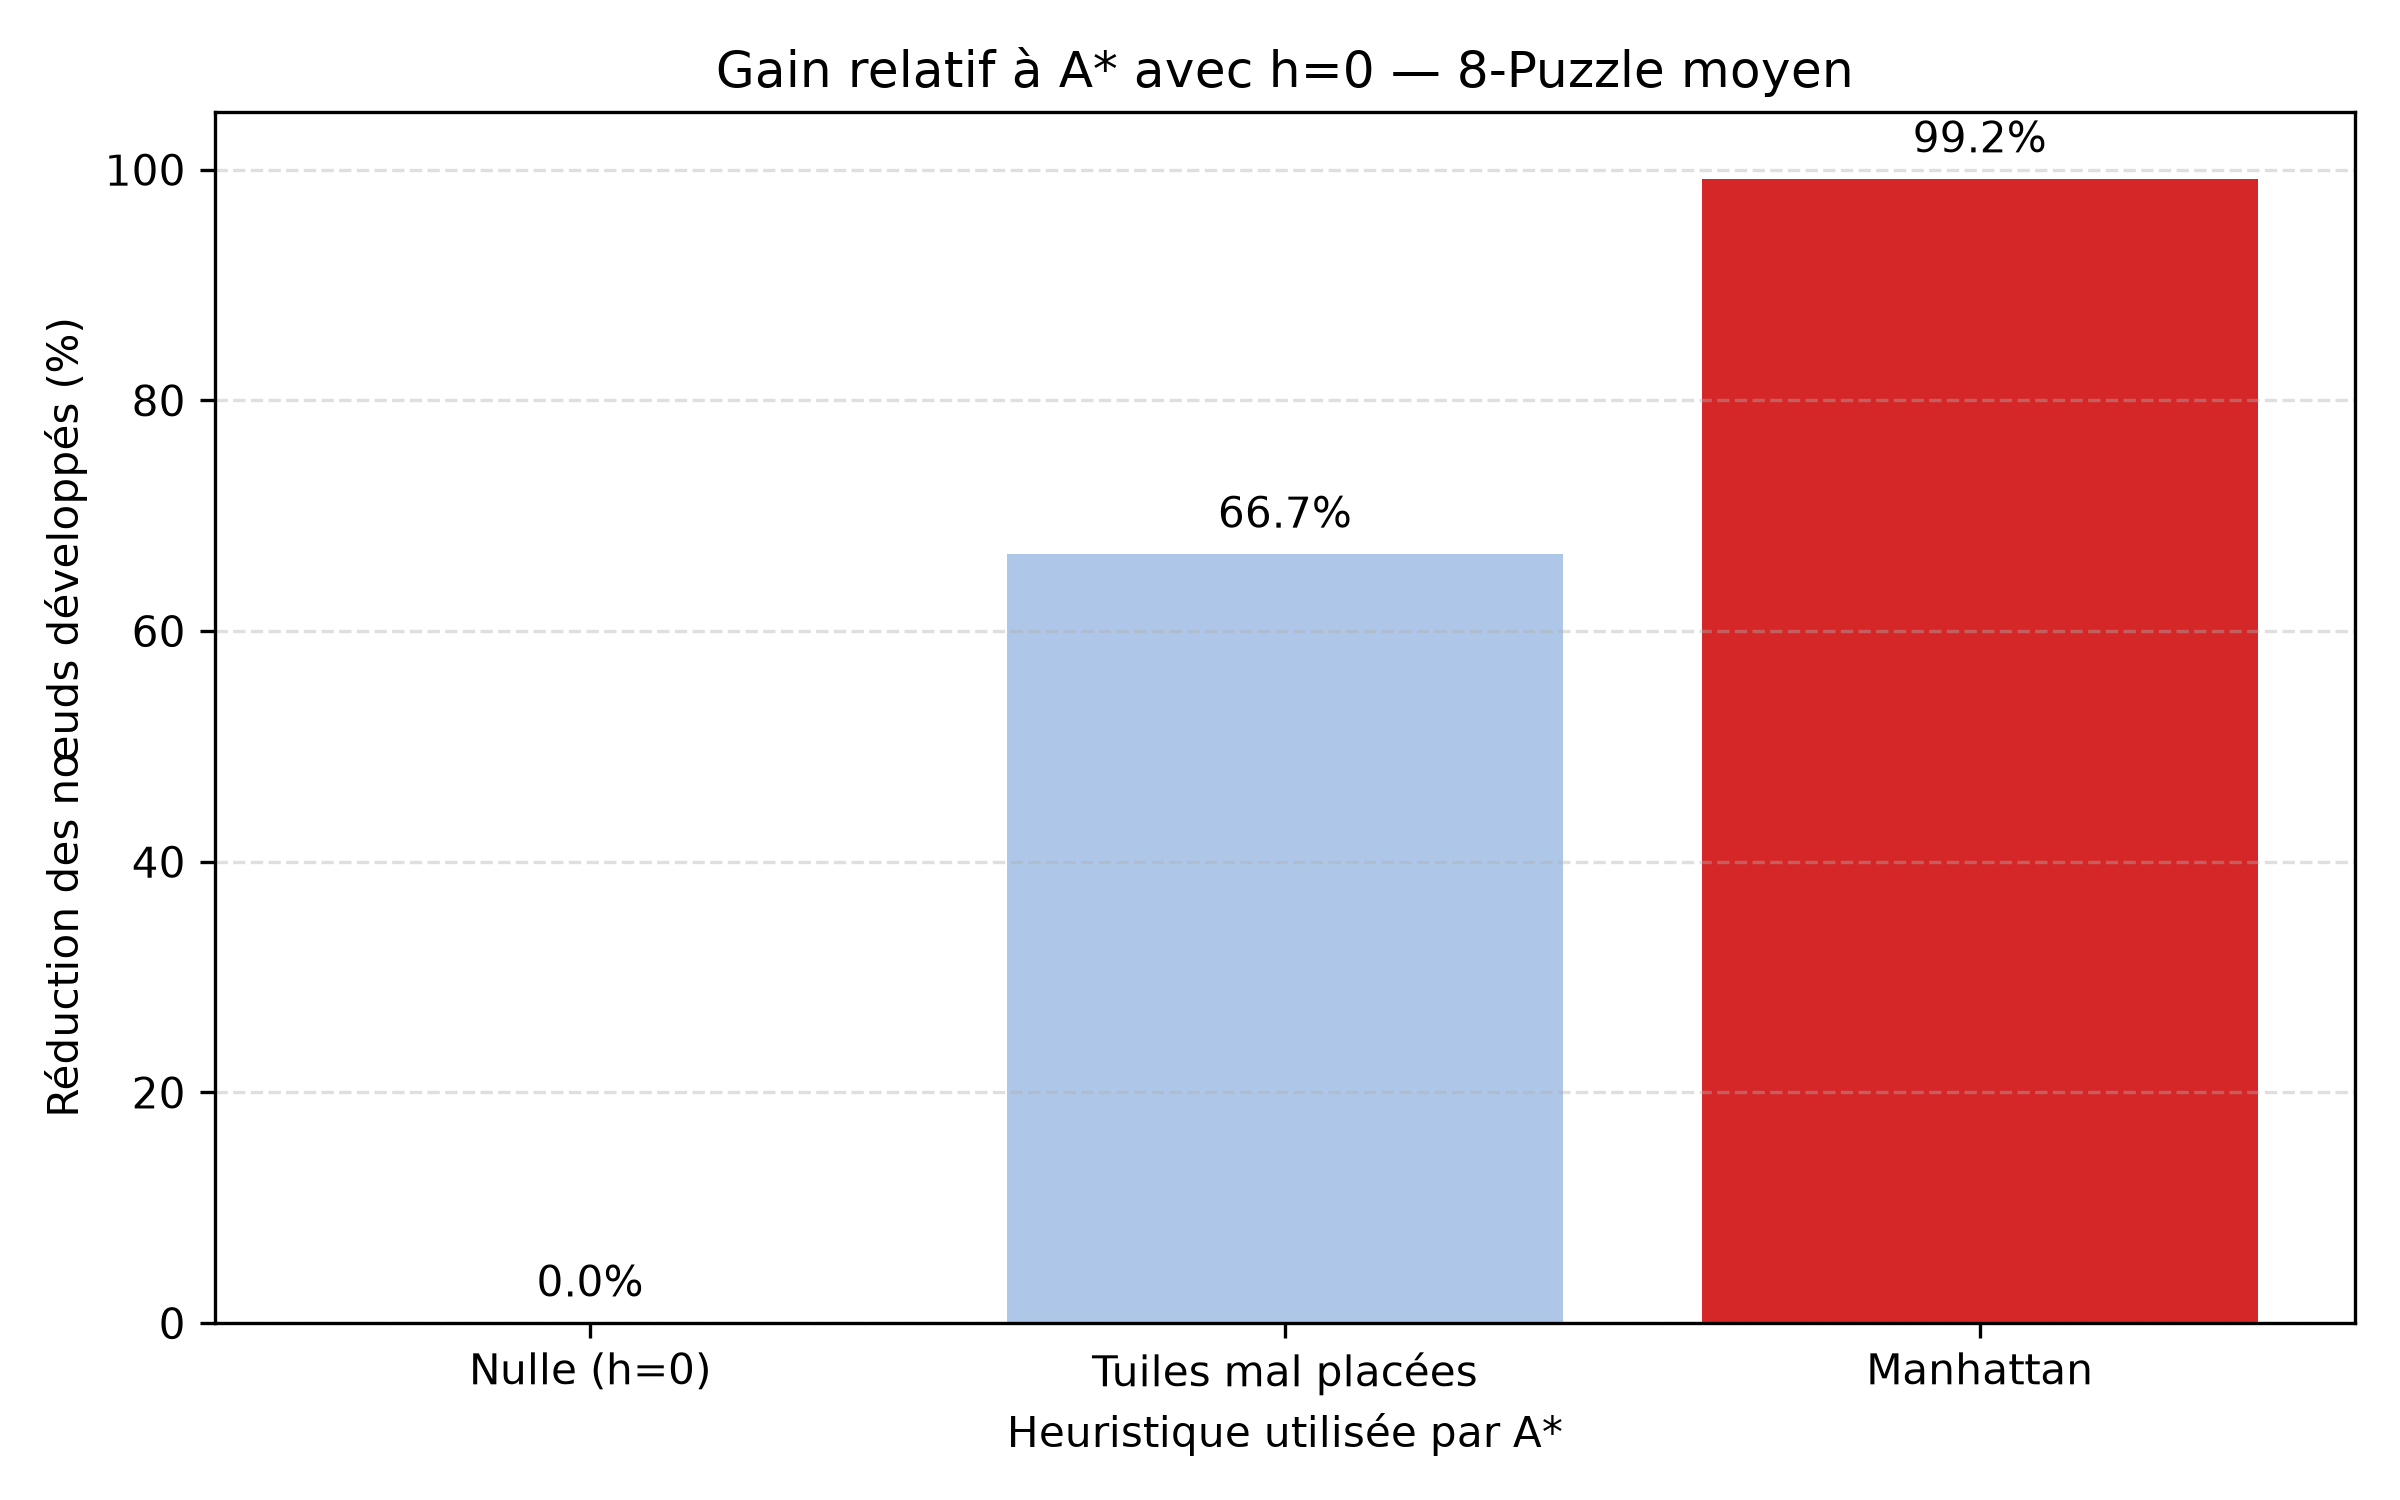
\includegraphics[width=0.78\textwidth]{figures/heuristiques_gain.png}
\caption{Réduction des noeuds expansés par rapport à \AStar{} avec
$h=0$.}
\label{fig:heuristiques-gain}
\end{figure}

\subsection{Jeu arithmétique : cas résolu et cas impossible}

Pour la cible 24, les quatre stratégies trouvent une solution en trois
opérations. Pour la cible 99 avec les nombres $1,1,1,1$, aucune solution n'est
trouvée et la frontière est entièrement épuisée. Chaque stratégie génère 97
noeuds et en développe 20 pour établir cet échec.

\begin{table}[H]
\centering
\caption{Résultats du jeu arithmétique en \GraphSearch{}.}
\label{tab:arithmetique-resultats}
\scriptsize
\begin{tabular}{llrrrrrr}
\toprule
\textbf{Instance} & \textbf{Stratégie} & \textbf{Résolue} &
\textbf{Coût / prof.} & \textbf{Gén.} & \textbf{Exp.} &
\textbf{OPEN max.} & \textbf{Temps (s)} \\
\midrule
Cible 24 & BFS & Oui & 3 / 3 & 881 & 114 & 321 & 0,007114 \\
Cible 24 & UCS & Oui & 3 / 3 & 1\,523 & 434 & 385 & 0,009120 \\
Cible 24 & Greedy & Oui & 3 / 3 & 558 & 284 & 45 & 0,004525 \\
Cible 24 & A* & Oui & 3 / 3 & 558 & 284 & 45 & 0,003879 \\
Cible 99 & BFS & Non & -- & 97 & 20 & 12 & 0,000560 \\
Cible 99 & UCS & Non & -- & 97 & 20 & 12 & 0,000545 \\
Cible 99 & Greedy & Non & -- & 97 & 20 & 10 & 0,000886 \\
Cible 99 & A* & Non & -- & 97 & 20 & 10 & 0,001107 \\
\bottomrule
\end{tabular}
\end{table}

\begin{figure}[H]
\centering
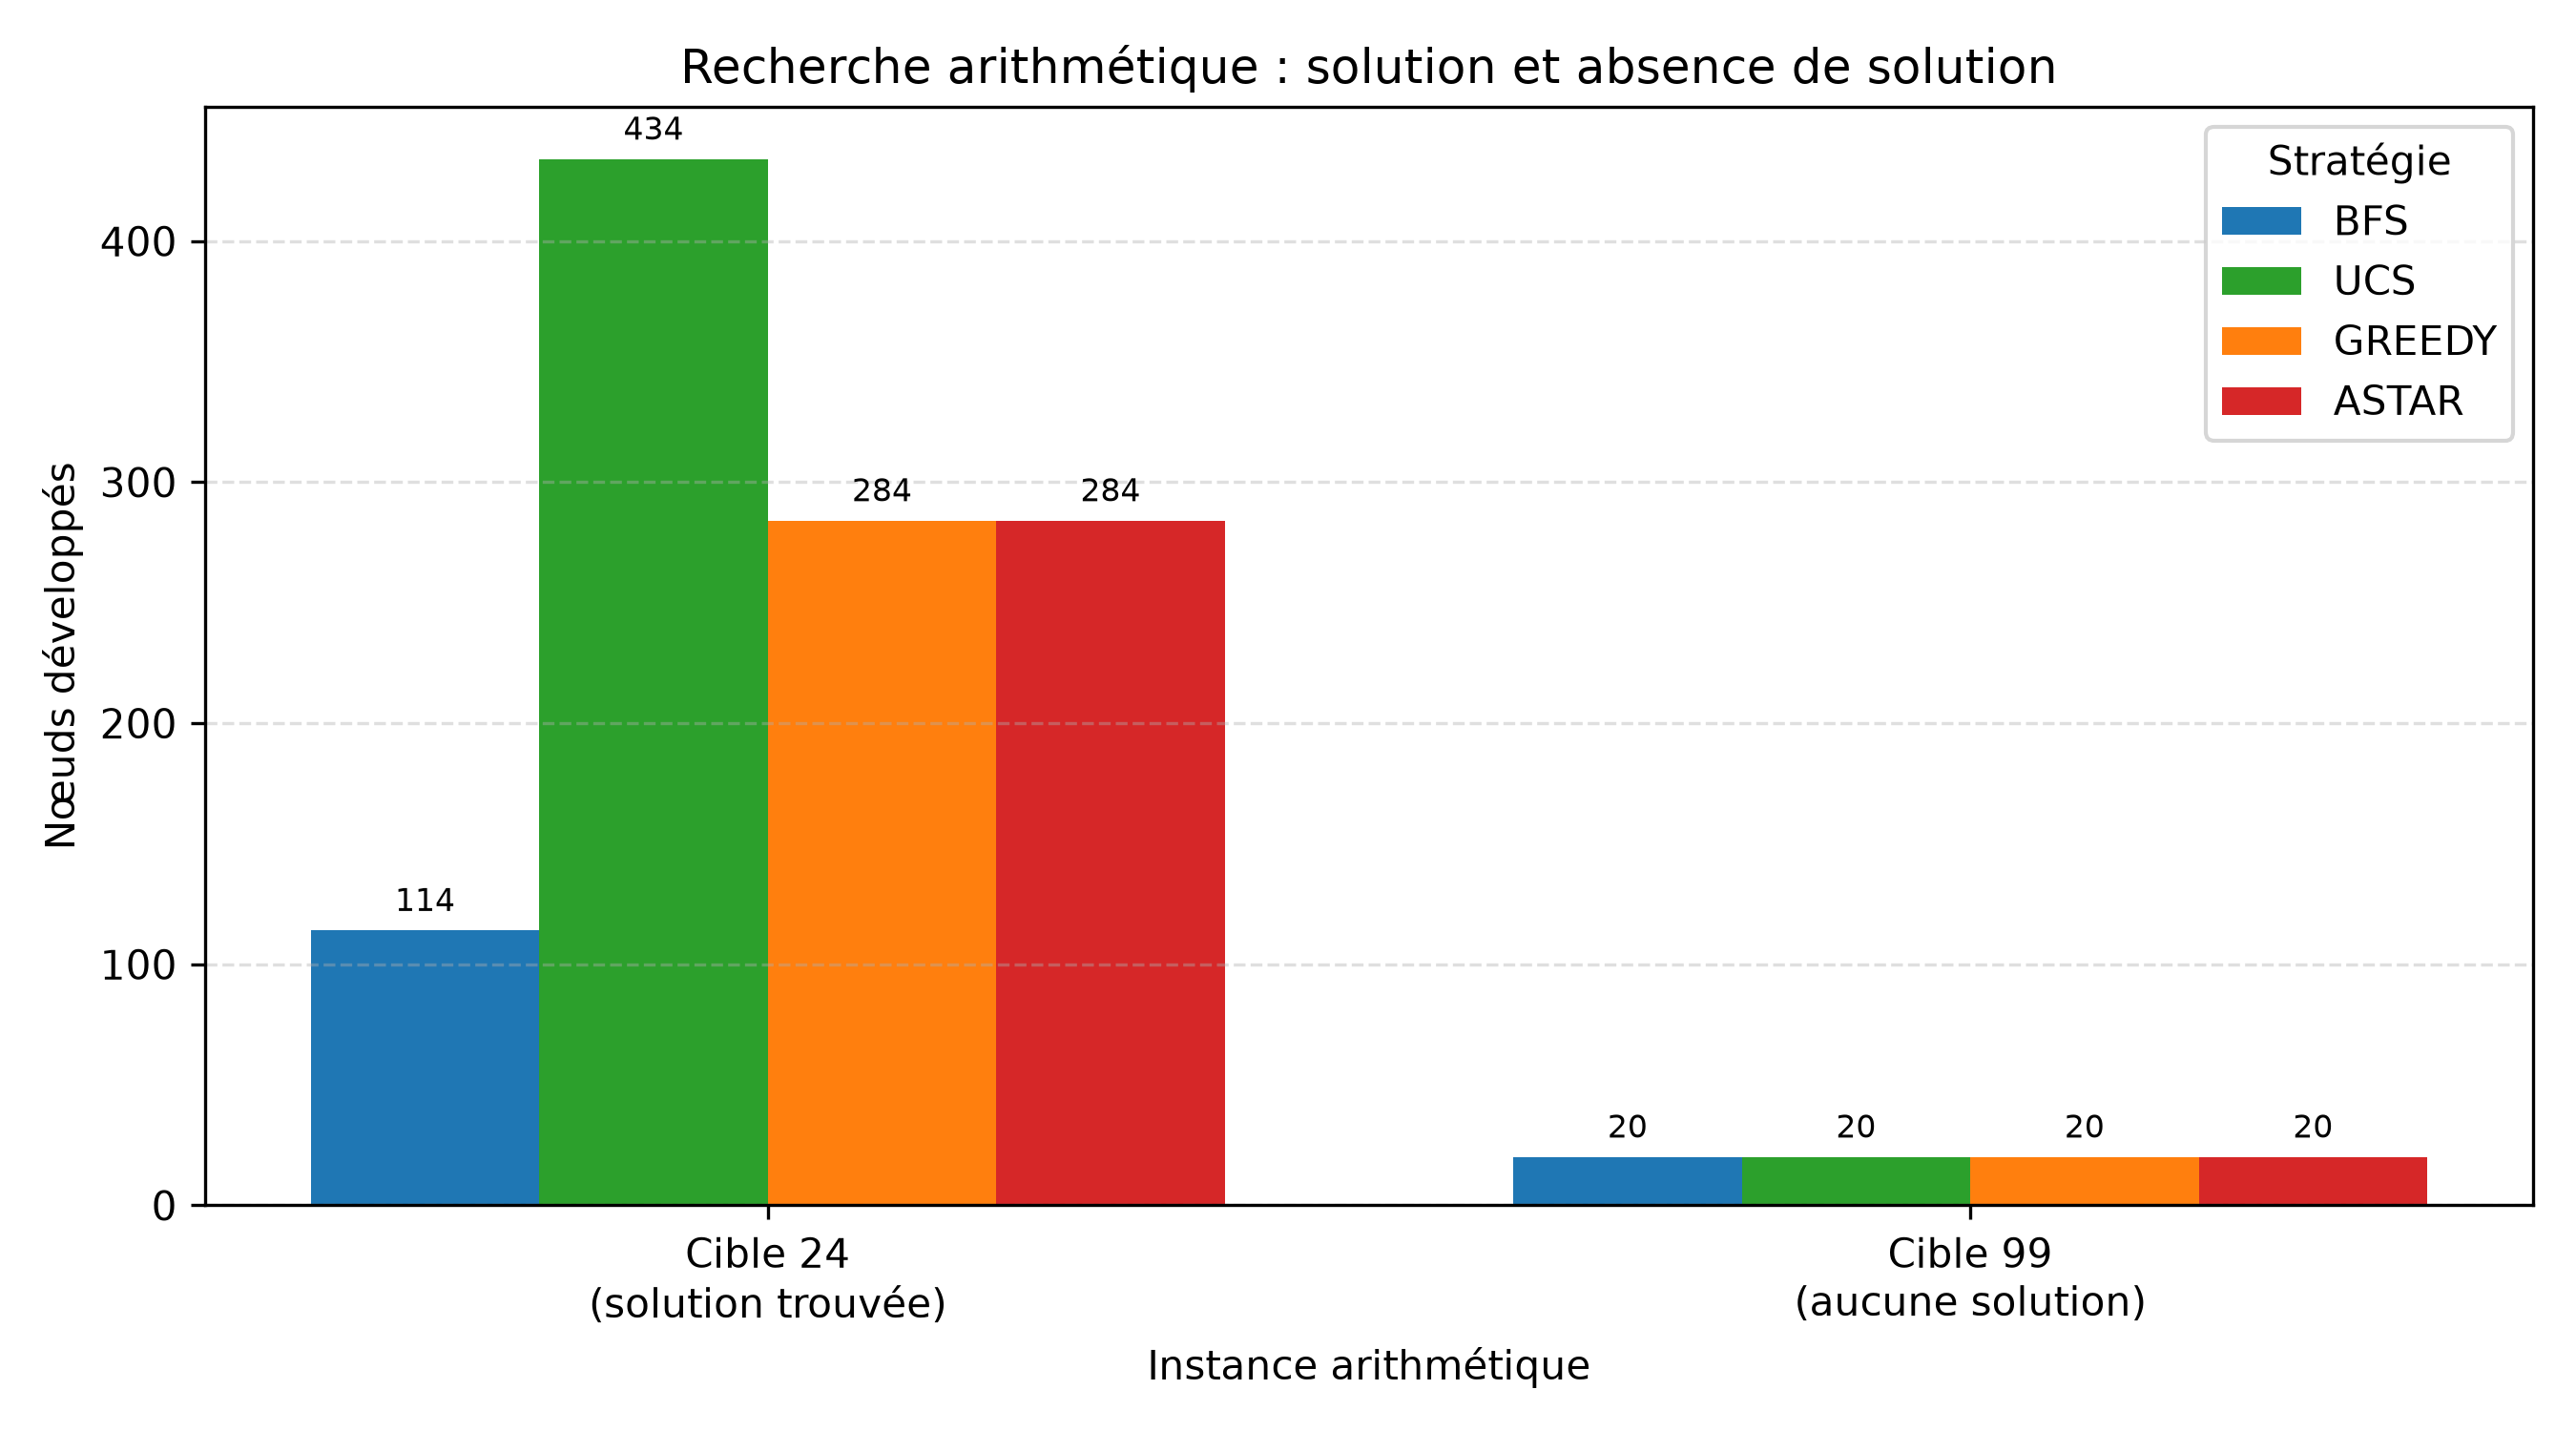
\includegraphics[width=0.82\textwidth]{figures/arithmetique_resultats.png}
\caption{Noeuds expansés pour le cas arithmétique résolu et le cas sans
solution.}
\label{fig:arithmetique-resultats}
\end{figure}

\subsection{Portée des résultats}

Ces mesures correspondent à un benchmark ciblé et ne remplacent pas les
expériences plus larges éventuellement présentées dans d'autres documents.
L'instance de labyrinthe pondéré testée donne le même coût à toutes les
stratégies; elle ne suffit donc pas à démontrer à elle seule que \BFS{} peut
être sous-optimale en présence de coûts variables. De même, une seule mesure
de temps par configuration ne permet pas d'établir une moyenne ou un intervalle
de confiance. Ces limites doivent être prises en compte dans l'interprétation.

\section{Discussion}

\subsection{Effet de l'heuristique}

Sur le 8-Puzzle moyen, les trois variantes d'\AStar{} trouvent une solution de
coût 28. La qualité de l'heuristique modifie toutefois fortement l'effort :
Manhattan développe 1\,440 noeuds, contre 59\,067 avec les tuiles mal placées
et 177\,134 avec $h=0$. Manhattan réduit ainsi le nombre de noeuds développés
de 99,2\,\% par rapport à la recherche sans information heuristique. Dans
cette expérience, le temps mesuré diminue également de 1,388574\,s à
0,014178\,s. Les temps étant mesurés une seule fois, cette dernière
comparaison reste indicative.

Greedy développe seulement 385 noeuds avec Manhattan, mais produit une
solution de 48 coups, alors que \AStar{} en trouve une de 28 coups. La
réduction du travail de recherche ne garantit donc pas l'optimalité de la
solution.

\subsection{Tree-Search contre Graph-Search}

Sur le labyrinthe pondéré, le nombre de noeuds expansés par \UCS{} passe de
596 en \TreeSearch{} à 15 en \GraphSearch{}; pour \BFS{}, il passe de 85 à
13. La mémorisation des états évite ici des développements répétés. L'ampleur
de l'amélioration varie néanmoins selon la stratégie et l'instance : sur le
labyrinthe simple, Greedy et \AStar{} développent chacun 4 noeuds dans les
deux modes.

\subsection{Coût de solution et effort}

Sur le trajet Gatineau--Baie-Comeau, \UCS{} et \AStar{} retournent un trajet
de 881,9\,km en 9 étapes, contre 912,7\,km en 6 étapes pour \BFS{} et Greedy.
La solution comportant le moins d'étapes n'est donc pas nécessairement celle
de coût minimal. Sur le 8-Puzzle moyen, Greedy illustre le même compromis :
385 développements pour une solution de 48 coups, au lieu des 1\,440
développements et 28 coups d'\AStar{}.

Le labyrinthe pondéré de ce benchmark constitue une limite importante : toutes
les stratégies y trouvent un chemin de coût 9 et de profondeur 6. Il ne
fournit donc pas un exemple où le coût de chemin distingue \BFS{} de \UCS{}.
Une instance pondérée supplémentaire, conçue pour offrir des chemins de
longueurs et de coûts différents, serait nécessaire pour mesurer directement
ce phénomène.

\subsection{Résolution des cas impossibles}

Pour le jeu arithmétique avec les nombres $1,1,1,1$ et la cible 99, chaque
stratégie termine l'exploration après 97 noeuds générés et 20 noeuds expansés,
sans solution. Il s'agit d'un échec après épuisement de l'espace d'états, et
non d'un arrêt dû à une limite de temps ou de mémoire. Le CSV du benchmark ne
contient pas de colonne de statut détaillé permettant de distinguer ces états
pour d'autres scénarios; le résultat de ce cas a été contrôlé pendant
l'exécution.

\subsection{Limites de l'évaluation}

\begin{itemize}
    \item Le benchmark ciblé couvre les cas indiqués dans la section
    \cref{sec:experiences}; il ne faut pas le confondre avec un éventuel
    benchmark antérieur portant sur davantage d'instances.
    \item Les temps correspondent à une seule exécution par configuration et
    peuvent varier selon l'environnement. Ils ne constituent pas des
    estimations statistiques.
    \item \code{max\_open} mesure la taille maximale de la frontière, pas la
    consommation mémoire totale.
    \item L'expérience heuristique porte sur une seule instance de 8-Puzzle.
    Des répétitions sur plusieurs états initiaux seraient nécessaires pour
    généraliser la conclusion.
\end{itemize}

\section{Conclusion}

Ce projet a permis de concevoir \AUSSI{}, un moteur générique de résolution de
problèmes basé sur la recherche dans un espace d'états. L'architecture repose
sur une séparation entre le moteur de recherche, les stratégies d'exploration,
les modes de gestion des duplications et les modèles spécifiques aux problèmes.

Le système prend en charge les labyrinthes, la navigation, le N-Puzzle et le
jeu arithmétique sans nécessiter de modification des algorithmes fondamentaux.
Les stratégies \BFS{}, \UCS{}, \Greedy{} et \AStar{} peuvent être sélectionnées
dynamiquement, tout comme les modes \TreeSearch{} et \GraphSearch{}.

Le benchmark ciblé confirme que la stratégie à privilégier dépend de
l'objectif. Sur le trajet routier testé, \UCS{} et \AStar{} trouvent le coût
minimal mesuré (881,9\,km), tandis que Greedy développe le moins de noeuds mais
renvoie un coût de 912,7\,km. Sur le 8-Puzzle moyen, \AStar{} avec Manhattan
trouve une solution de 28 coups en développant 1\,440 noeuds, contre 177\,134
avec $h=0$. Enfin, sur le labyrinthe pondéré, \GraphSearch{} réduit fortement
les développements de \UCS{} par rapport à \TreeSearch{} (15 contre 596).

Ces résultats restent limités aux instances décrites dans le protocole. Les
temps n'ont été mesurés qu'une fois par configuration, et le labyrinthe
pondéré ne distingue pas les stratégies par le coût obtenu. Des expériences
répétées sur davantage d'instances pondérées et de configurations du N-Puzzle
permettraient de renforcer les conclusions.

Les améliorations futures possibles comprennent l'ajout de nouvelles stratégies
de recherche, des heuristiques plus avancées, une interface graphique et un
module de génération automatique d'instances de problèmes.

\end{document}
